% !TEX root = handbook-physics.tex
% !TEX TS-program = pdflatex
% !TEX encoding = UTF-8 Unicode






\chapter{Polarization of Light}
\label{ch-35}
\zhtitle{光的偏振}

\section{Polarization of Light in Reflection and Refraction
at the Interface Between Two Dielectric Media}
\label{sec-35.1} 
\zhtitle{两种电介质分界面上的反射与折射中的光偏振}


\subsection{}\label{35.1.1} Light emitted by ordinary (nonlaser) sources is made up of a set of a great many plane polarized wave trains, or packets \ssect{32.1.3}, whose electric vectors $\vb{E}$ vary along all possible directions perpendicular to the ray \ssect{30.2.1}. Light is said to be
\redem{natural}, or \redem{unpolarized}, if not one of the above-indicated directions of vibration is predominant. In natural light, the resultant strength $\vb{E}$ oscillates at each point of the field in a direction that rapidly and randomly varies in a plane perpendicular to the ray.
\zhpar{普通（非激光）光源发出的光由大量平面偏振波列（或称波包\ssect{32.1.3}）组成，这些波列的电矢量 $\vb{E}$ 沿垂直于光线\ssect{30.2.1}的所有可能方向振动。若在这些振动方向中没有任何一个占优势，则称该光为\redem{自然光}，或\redem{非偏振光}。在自然光中，场中每一点的合场强 $\vb{E}$ 在垂直于光线的平面内振动，其方向快速而无规则地变化。}

Light is said to be \redem{partially polarized} if in it there is a predominant direction of oscillation of vector $\vb{E}$. Partially polarized light can be regarded as a collection (``mixture'') of natural and linearly polarized light, simultaneously propagating in a single direction.
\zhpar{若光中存在占优势的电矢量 $\vb{E}$ 振动方向，则称该光为\redem{部分偏振光}。部分偏振光可以看作是沿同一方向同时传播的自然光与线偏振光的“混合物”。}

\subsection{}\label{35.1.2} The \redem{polarization of light} is the separation of linearly polarized light out of natural or partially polarized light. Special devices, called \redem{polarizers}, are used for this purpose. Their principle
of operation is based on the polarization of light upon
being reflected or refracted by the interface between two dielectric media, as well as on the phenomenon of birefringence \ssect{35.2.1} and dichroism \ssect{35.2.10}. The same devices can be utilized as \redem{analyzers}, i.e. devices to determine the kind and degree of polarization of light.
\zhpar{\redem{光的偏振}是指从自然光或部分偏振光中分离出线偏振光。为此目的，需要使用称为\redem{起偏器}的专用器件。这类器件的工作原理基于光在两种电介质分界面上反射或折射时产生的偏振现象，以及双折射\ssect{35.2.1}和二色性\ssect{35.2.10}现象。同样的器件也可以用作\redem{检偏器}，即用来确定光的偏振类型和偏振程度的器件。}

\begin{marginfigure}%[-3cm] 
\centering
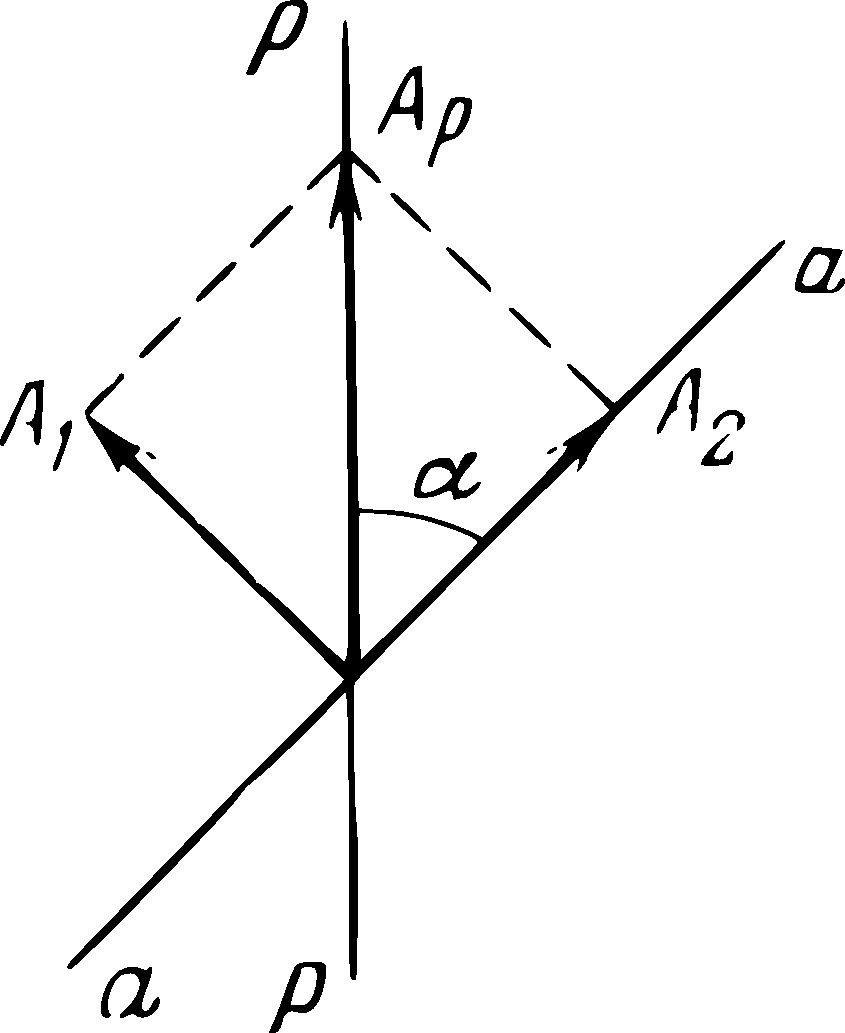
\includegraphics[width=0.8\textwidth]{figs/ch-35/fig-35-01.pdf}
\sidecaption{Analysing linearly polarized light.\zhcap{线偏振光的检偏。}\label{fig-35-01}}
\end{marginfigure}


Assume that linearly polarized light, whose electric vector $\vb{E}_{p}$ is along the line $p$-$p$ and oscillates with the amplitude $A_{p}$, falls on the analyzer perpendicularly to the plane of \figr{fig-35-01}. Assume further that the electric vector $\vb{E}_{a}$ of the light passed by the analyzer is along line $a$-$a$, which makes the angle $\alpha$ with line $p$-$p$. The incident light can be represented in the form of two waves, linearly polarized in mutually perpendicular planes \ssect{31.1.8}. The wave whose electric vector $\vb{E}_{1}$ oscillates along the direction perpendicular to $a$-$a$, with the amplitude $A_{1} = A_{p} \sin \alpha$, cannot pass through the analyzer. But the other wave, whose electric vector $\vb{E}_{2}$ oscillates along the direction of $a$-$a$, with the amplitude $A_{2} = A_{p} \cos \alpha$ passes completely through the analyzer. Consequently, the amplitude of the light emerging from the analyzer is
\zhpar{设线偏振光的电矢量 $\vb{E}_{p}$ 沿直线 $p$-$p$ 方向振动，振幅为 $A_{p}$，该光垂直于\figr{fig-35-01}所在的平面入射到检偏器上。设透过检偏器的光的电矢量 $\vb{E}_{a}$ 沿直线 $a$-$a$ 方向，该直线与直线 $p$-$p$ 成夹角 $\alpha$。入射光可以表示为两个分别在相互垂直平面内线偏振的波\ssect{31.1.8}。电矢量 $\vb{E}_{1}$ 沿垂直于 $a$-$a$ 的方向振动、振幅为 $A_{1} = A_{p} \sin \alpha$ 的波不能透过检偏器；而电矢量 $\vb{E}_{2}$ 沿 $a$-$a$ 方向振动、振幅为 $A_{2} = A_{p} \cos \alpha$ 的波则完全透过检偏器。因此，从检偏器射出的光的振幅为}
\begin{equation*}%
A_{a} = A_{2} = A_{p} \cos \alpha.
\end{equation*}
The intensities $I_{a}$ and $I_{p}$ of the linearly polarized light incident on and emerging from the analyzer, respectively, are related by the \redem{Malus law}:
\zhpar{入射到检偏器上和从检偏器射出的线偏振光的强度分别为 $I_{a}$ 和 $I_{p}$，二者之间由\redem{马吕斯定律}相联系：}
\begin{equation*}%
I_{a}= I_{p} \cos^{2} \alpha.
\end{equation*}
The \redem{principal plane of a polarizer} (or \redem{analyzer}) is the plane of polarization [plane of oscillation, according to previous terminology
\ssect{31.1.7}] of light passed through the polarizer (or analyzer).
\zhpar{起偏器（或检偏器）的\redem{主平面}是指透过该起偏器（或检偏器）的光的偏振面〔按照以前的术语，即振动面，见\ssect{31.1.7}〕。}

\subsection{}\label{35.1.3} In investigating the laws of light polarization as a result of reflection and refraction of natural light, the light can be conveniently dealt with as a combination of linearly polarized waves, of equal intensities, of two types: $s$- and $p$-waves \ssect{31.5.4}.
\zhpar{在研究自然光经反射和折射后的偏振规律时，可以方便地把自然光看作两种类型、强度相等的线偏振波的组合，即 $s$ 波和 $p$ 波\ssect{31.5.4}。}

The reflection coefficient \ssect{31.5.6} of the $s$-waves ($R_{s}$) is always greater than that ($R_{p}$) of the $p$-waves. Therefore, in contrast to incident natural light, reflected and transmitted (refracted) light is partially polarized. Oscillations of the electric field vector
$\vb{E} $ of the $s$-type (perpendicular to the plane of incidence) predominate in reflected light, whereas oscillations of the $p$-type (in the plane of incidence) predominate in transmitted light.
\zhpar{$s$ 波的反射系数\ssect{31.5.6}（$R_{s}$）总是大于 $p$ 波的反射系数（$R_{p}$）。因此，与入射的自然光不同，反射光和透射（折射）光都是部分偏振光。反射光中以垂直于入射面的 $s$ 型电场矢量 $\vb{E}$ 振动占优势，而透射光中则以位于入射面内的 $p$ 型振动占优势。}

\redem{Brewster's law} states that reflected light is completely linearly polarized at the angle of incidence $i = i_{Br}$, complying with the condition $\tan i_{Br} =  n_{21}$, where $n_{21}$ is the relative refractive index of a medium reflecting light.
\zhpar{\redem{布儒斯特定律}指出：当入射角 $i = i_{Br}$ 满足条件 $\tan i_{Br} = n_{21}$ 时，反射光是完全线偏振光，式中 $n_{21}$ 为反射光所在介质的相对折射率。}

The angle $i_{Br}$ is called \redem{Brewster's} angle. When $i = i_{Br}$, the reflected and refracted rays are perpendicular to each other and the the reflection coefficient of the $p$-wave is $R_{p} = 0$ \ssect{31.5.6}. Hence, only $s$-type waves are reflected. But their reflection coefficient is considerably less than unity (about 0.15 for glass). Thus, the transmitted light is only partially polarized.
\zhpar{角 $i_{Br}$ 称为\redem{布儒斯特角}。当 $i = i_{Br}$ 时，反射光线与折射光线相互垂直，且 $p$ 波的反射系数为 $R_{p} = 0$\ssect{31.5.6}。因此只有 $s$ 型波被反射。但其反射系数远小于 1（对玻璃约为 0.15），所以透射光只是部分偏振光。}

\subsection{}\label{35.1.4} Polarization of transmitted light can be enhanced by subjecting the light to a number of consecutive reflections and refractions. This is done in a stack consisting of several identical and parallel plates of some transparent dielectric (for instance, glass), set at the Brewster angle to the incident light beam.
\zhpar{通过让光经历多次连续的反射和折射，可以增强透射光的偏振程度。为此，可采用由若干块相同且彼此平行的透明电介质（例如玻璃）薄片组成的片堆，并使其与入射光束成布儒斯特角放置。}

If the number of plates in the stack is sufficiently large, then the light passing through the stack is found to be practically linearly polarized ($p$-type). In the absence of light absorption in the stack, the intensities $I_{s}$ and $I_{p}$ of the reflected and transmitted linearly polarized light are the same and equal to one-half of the intensity $I_{0}$ of the incident natural light. Thus
\zhpar{若片堆中的薄片数目足够多，则透过片堆的光实际上是线偏振光（$p$ 型）。在没有光吸收的片堆中，反射和透射的线偏振光的强度 $I_{s}$ 与 $I_{p}$ 相等，且都等于入射自然光强度 $I_{0}$ 的一半。因此}
\begin{equation*}%
I_{s} = I_{p} = \frac{1}{2} I_{0}.
\end{equation*}



\begin{marginfigure}%[-3cm] 
\centering
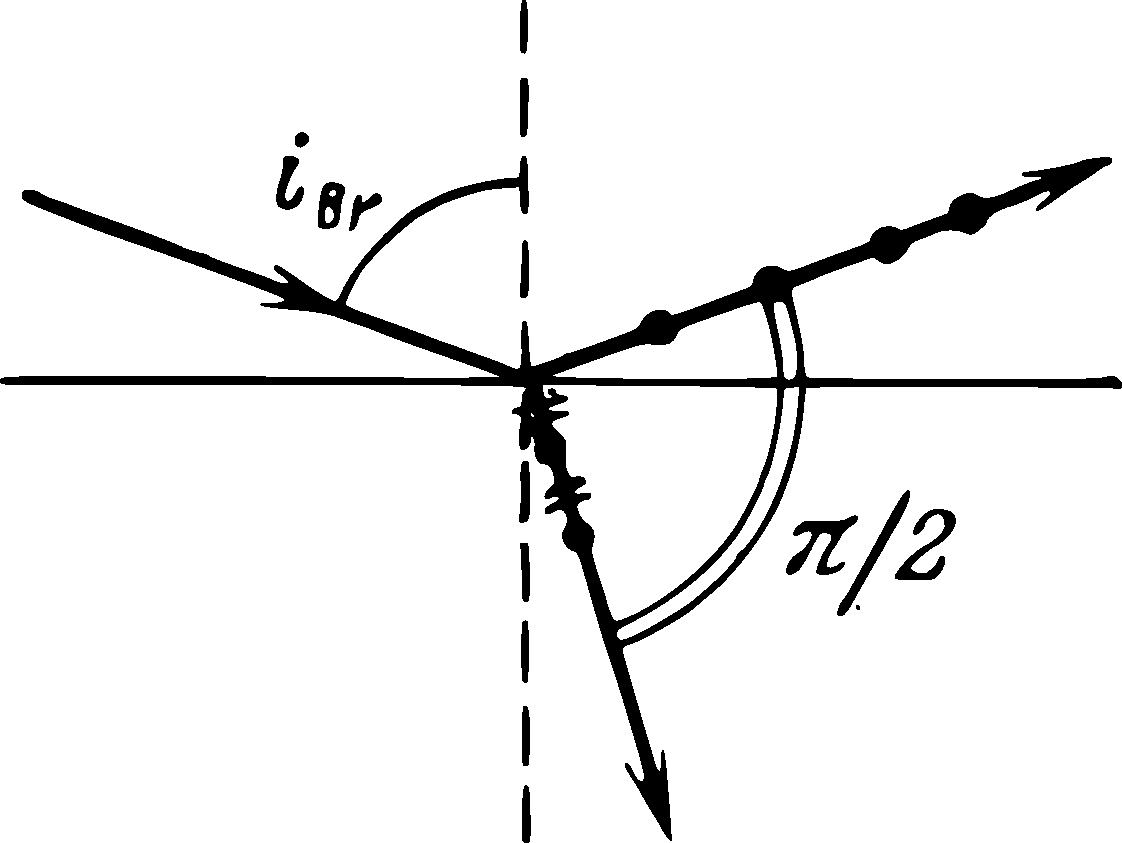
\includegraphics[width=0.8\textwidth]{figs/ch-35/fig-35-02.pdf}
\sidecaption{Polarization of light on refraction and reflection.\zhcap{光在折射和反射时的偏振。}\label{fig-35-02}}
\end{marginfigure}

\subsection{}\label{35.1.5} According to the conceptions of classical electron theory, the formation of the reflected wave is due to the secondary waves emitted by the molecules, the
oscillators of the light reflecting medium \ssect{34.1.3}. Oscillators (vibrating electric dipoles), whose axis is perpendicular to the plane of incidence, correspond to a wave of the $s$-type. These oscillators are shown in \figr{fig-35-02}
by black dots on the refracted and reflected rays. As is evident from the polar directional diagram (\figr{fig-35-04}), such oscillators should radiate intensively in all directions lying in the plane of incidence, i.e. they should participate in the formation of both the reflected and the refracted $s$-waves.
\zhpar{根据经典电子理论，反射波是由反射光所在介质中作为振子的分子所发出的次级波形成的\ssect{34.1.3}。轴线垂直于入射面的振子（即振动的电偶极子）对应于 $s$ 型波，它们在\figr{fig-35-02}中以折射光线和反射光线上的黑点表示。由极坐标方向图（\figr{fig-35-04}）可见，这类振子应在入射面内的所有方向上强烈辐射，即它们既参与反射 $s$ 波的形成，也参与折射 $s$ 波的形成。}




Oscillators, whose axis lies in the plane of incidence and is
perpendicular to the refracted ray (shown in \figr{fig-35-02} by transverse dashes), correspond to a wave of the $p$-type. Oscillators do not radiate along their axis (\figr{fig-35-04}), and at $i = i_{Br}$ the reflected ray is perpendicular to the refracted one, thereby being parallel to the axes of these oscillators. Hence, at $i = i_{Br}$ these oscillators do not radiate in the direction of the reflected ray, making no contribution to the reflected wave. Consequently, the reflected light is completely linearly polarized ($s$-type
waves).
\zhpar{轴线位于入射面内且垂直于折射光线的振子（在\figr{fig-35-02}中以短横线表示）对应于 $p$ 型波。振子不沿其轴线方向辐射（见\figr{fig-35-04}）。当 $i = i_{Br}$ 时，反射光线与折射光线相互垂直，因而反射光线与这些振子的轴线平行。因此，在 $i = i_{Br}$ 时，这些振子不沿反射光线方向辐射，对反射波没有贡献。由此可知，反射光是完全线偏振的（$s$ 型波）。}

\section{Birefringence (Double Refraction)}
\label{sec-35.2} 
\zhtitle{双折射（重折射）}


\begin{marginfigure}%[-3cm] 
\centering
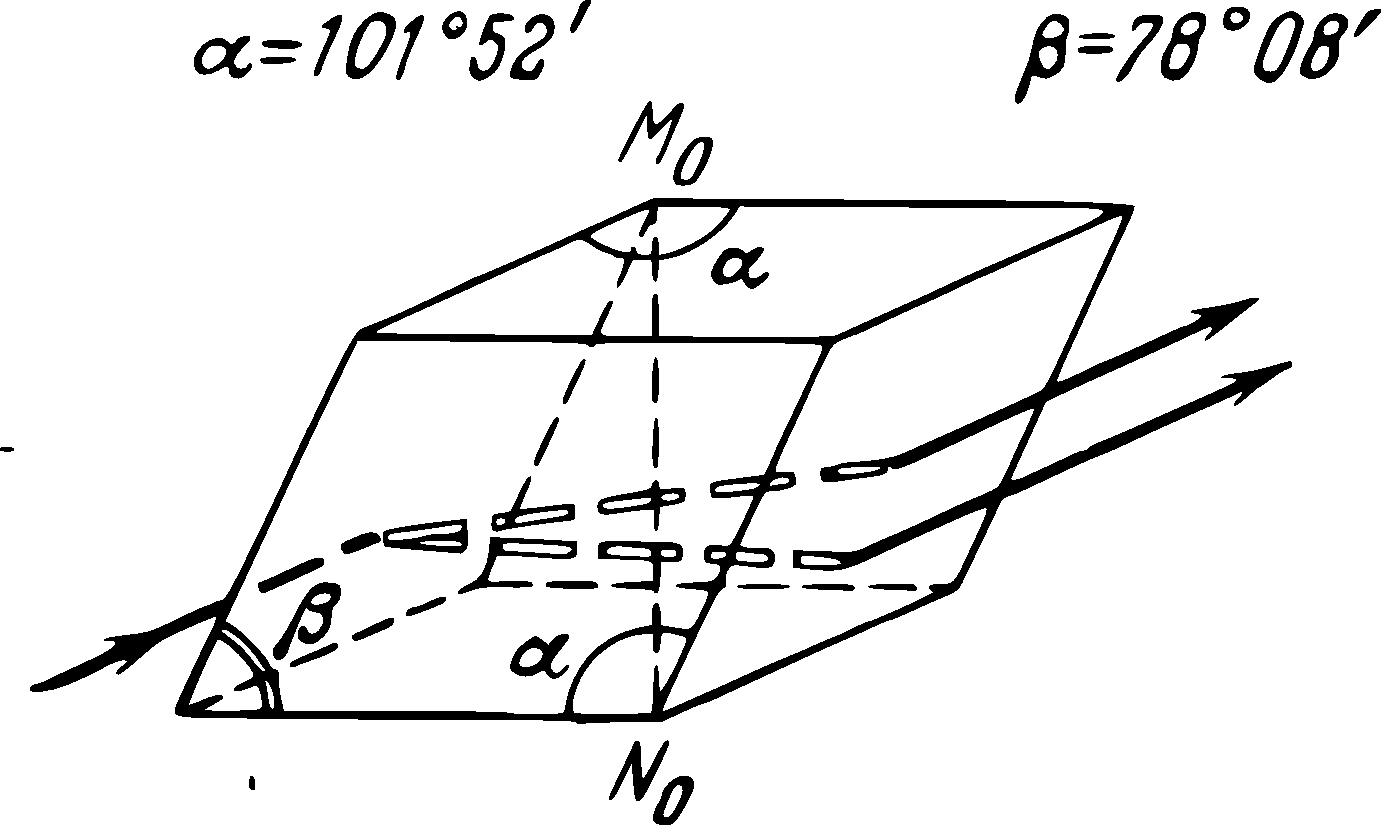
\includegraphics[width=\textwidth]{figs/ch-35/fig-35-03.pdf}
\sidecaption{The birefringence of light in a crystal
of Iceland spar (\ce{CaCO3}).\zhcap{光在冰洲石（\ce{CaCO3}）晶体中的双折射。}\label{fig-35-03}}
\end{marginfigure}



\subsection{}\label{35.2.1} Most crystals are optically anisotropic \ssect{30.1.6}. Their relative dielectric permittivity (dielectric constant) and refractive index depend on the direction of the electric vector $\vb{E}$ of the light wave. Observed in optically anisotropic crystals is the phenomenon of \redem{double refraction}, or \redem{birefringence}, which consists in the splitting of a light ray, falling on a surface of the crystal, into two refracted rays. The birefringence of light in a crystal
of Iceland spar (\ce{CaCO3}) is illustrated in \figr{fig-35-03}.
\zhpar{大多数晶体是光学各向异性的\ssect{30.1.6}。它们的相对电容率（介电常量）和折射率取决于光波电矢量 $\vb{E}$ 的方向。在光学各向异性晶体中可以观察到\redem{双折射}，或称\redem{重折射}现象，即入射到晶体表面上的一束光线分裂为两束折射光线。冰洲石（\ce{CaCO3}）晶体中光的双折射如\figr{fig-35-03}所示。}

\subsection{}\label{35.2.2} The \redem{optic axis of a crystal} is the direction in an optically anisotropic crystal along which light propagates without undergoing birefringence. It is necessary to underline that the optic axis of a crystal is no single special straight line similar, for instance, to the axis of symmetry of a body. It only characterizes a certain \redem{direction} in the crystal and can be passed through any point of the crystal.
\zhpar{\redem{晶体光轴}是指光学各向异性晶体中光沿其传播而不发生双折射的方向。需要强调的是，晶体光轴并不是像物体对称轴那样的某一条特定直线。它只表示晶体中的某一\redem{方向}，并且可以经过晶体中的任意一点。}

Depending upon their type of symmetry, optically anisotropic
crystals can be either \redem{uniaxial} or \redem{biaxial}, i.e. they can have either one or two optic axes. An example of a uniaxial crystal is Iceland spar, whose optic axis coincides in direction with the diagonal $M_{0}N_{0}$ of the crystal (\figr{fig-35-03}).
\zhpar{根据对称性的类型，光学各向异性晶体可以是\redem{单轴}晶体或\redem{双轴}晶体，即分别具有一个或两个光轴。冰洲石是单轴晶体的一个例子，其光轴方向与晶体的对角线 $M_{0}N_{0}$ 一致（见\figr{fig-35-03}）。}

The \redem{principal plane} (or \redem{principal section}) \redem{of a uniaxial crystal} for a certain ray is the plane passing through this ray and intersecting the optic axis.
\zhpar{对于某一光线，\redem{单轴晶体的主平面}（或称\redem{主截面}）是指通过该光线并与光轴相交的平面。}


\begin{marginfigure}%[-3cm] 
\centering
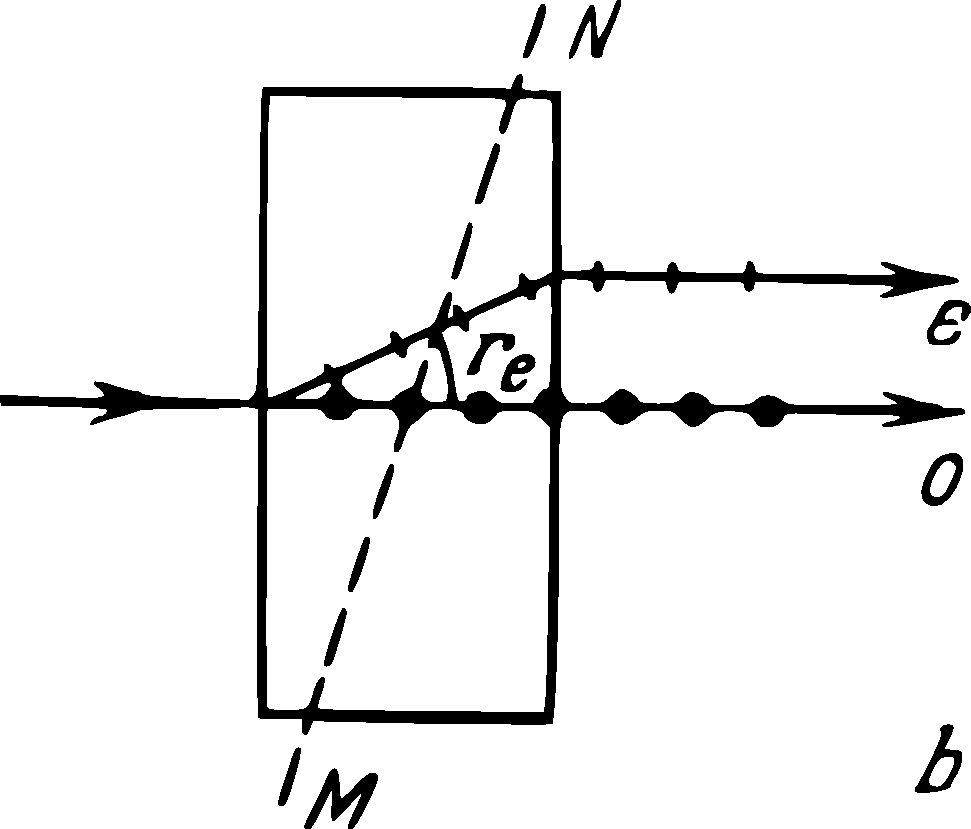
\includegraphics[width=\textwidth]{figs/ch-35/fig-35-04.pdf}
\sidecaption{The ordinary and extraordinary rays.\zhcap{寻常光线与非常光线。}\label{fig-35-04}}
\end{marginfigure}


\subsection{}\label{35.2.3} In a uniaxial crystal, one of the rays formed in birefringence (double refraction) obeys the ordinary laws of light refraction \ssect{31.5.3}. It lies in the plane of incidence and complies with Snell's law. It is therefore called the \redem{ordinary}, or \redem{$O$ ray}. The
second ray is called the \redem{extraordinary} or \redem{$E$ ray} because it generally does not lie in the plane of incidence and does not obey Snell's law. 
\zhpar{在单轴晶体中，双折射产生的两束光线之一遵循光的普通折射定律\ssect{31.5.3}：它位于入射面内并服从斯涅耳定律，因此称为\redem{寻常光}，或\redem{$O$ 光}。另一束光线称为\redem{非常光}，或\redem{$E$ 光}，因为它一般不位于入射面内，也不服从斯涅耳定律。}

For example, even in the case of normal incidence of light on a plate cut from a uniaxial crystal, the extraordinary ray is refracted (\figr{fig-35-04}). Its refractive angle $r_{e}$ depends on how the surface of the plate is oriented with respect to the optic axis of the crystal. It may be equal to zero only in two cases:
\zhpar{例如，即使光垂直入射到由单轴晶体切出的平板上，非常光线仍会发生折射（见\figr{fig-35-04}）。其折射角 $r_{e}$ 取决于平板表面相对于晶体光轴的取向，只有在以下两种情况下它才可能等于零：}
\begin{enumerate}[label=(\alph*)]
\item if the surface of the plate is perpendicular to the optic axis (light propagates in the plate along the optic axis and is thereby not subject to birefringence);
\zhpar{平板表面垂直于光轴（光沿光轴在平板中传播，因而不发生双折射）；}
\item if the surface of the plate is parallel to the optic axis (light propagates in the plate perpendicular to the optic axis).
\zhpar{平板表面平行于光轴（光在平板中垂直于光轴传播）。}
\end{enumerate}
In a biaxial crystal both refracted rays behave like extraordinary ones.
\zhpar{在双轴晶体中，两束折射光线的行为都与非常光线相同。}

\subsection{}\label{35.2.4} Birefringence indicates that a light wave incident on an optically anisotropic crystal produces two waves, propagating through the crystal, generally in different directions. In a uniaxial crystal, they are called the \redem{ordinary} and \redem{extraordinary} waves. The ordinary and extraordinary rays indicate the directions of the Umov-Poynting vectors \ssect{31.2.3} of the corresponding
waves in the crystal, i.e. the direction of energy transfer
by these waves.
\zhpar{双折射表明，入射到光学各向异性晶体上的光波会在晶体中产生两个波，它们一般沿不同方向传播。在单轴晶体中，它们分别称为寻常波和非常波。寻常光线和非常光线分别指示了相应波在晶体中的乌莫夫-坡印廷矢量\ssect{31.2.3}的方向，即这些波传递能量的方向。}

\begin{marginfigure}%[-3cm] 
\centering
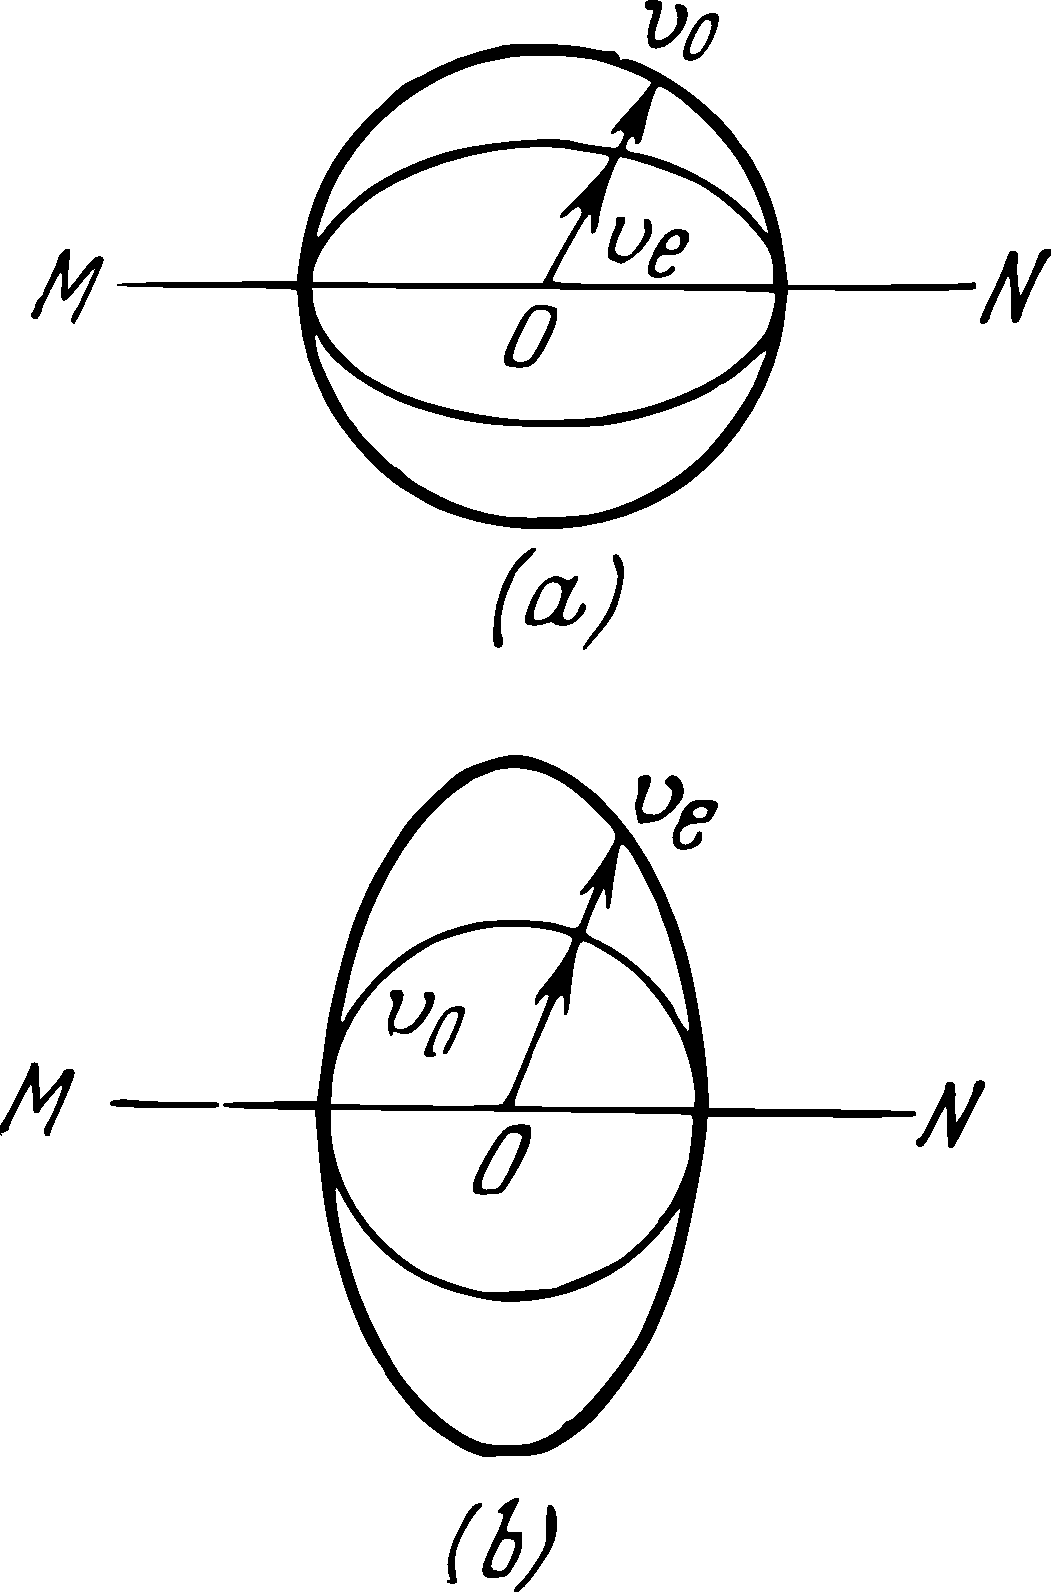
\includegraphics[width=0.8\textwidth]{figs/ch-35/fig-35-05.pdf}
\sidecaption{The velocity of ordinary and extraordinary rays in an anisotropic crystal.\zhcap{寻常光线与非常光线在各向异性晶体中的速度。}\label{fig-35-05}}
\end{marginfigure}


The ordinary and extraordinary waves are linearly polarized
\ssect{31.1.7}.\sidenote[][-4cm]{Frequently, mention is made of linear polarization of the ordinary and extraordinary rays, actually meaning the polarization of the waves corresponding to them.} In the ordinary wave, vector $\vb{E}$ is perpendicular to the principal plane of the crystal for the ordinary ray. The
electric vector $\vb{E}$ of the extraordinary wave lies in the principal plane of the crystal for the extraordinary ray. The directions of vectors $\vb{E}$ in the ordinary and extraordinary waves are conditionally shown in \figr{fig-35-04} by black dots on the ordinary ray and transverse dashes on the extraordinary ray (it is assumed that both rays, and optic axis $MN$ intersecting them, lie
in the plane of the figure).
\zhpar{寻常波和非常波都是线偏振的\ssect{31.1.7}。在寻常波中，电矢量 $\vb{E}$ 垂直于寻常光线所在的晶体主平面；非常波的电矢量 $\vb{E}$ 位于非常光线所在的晶体主平面内。两种波的电矢量方向在\figr{fig-35-04}中示意性地给出：寻常光线上以黑点表示，非常光线上以短横线表示（假定两条光线以及与之相交的光轴 $MN$ 都位于图面内）。}
\zhpar{注：常提到寻常光线和非常光线的线偏振，实际上指的是与它们对应的波的偏振。}




\subsection{}\label{35.2.5} The \redem{ray velocity of the wave}, or simply \redem{ray velocity}, in an optically anisotropic crystal is the velocity $\vb{v}$ of energy transfer by the wave. In a uniaxial crystal, the \redem{velocity $\vb{v}_{o}$ of the ordinary ray} is numerically equal in all directions: $v_{o} = c/n_{o}$, where $c$ is the velocity of light in free space (or in vacuum), and $n_{o} = \text{const}.$ is the \redem{refractive index of the crystal for the ordinary ray}. Accordingly, the \redem{velocity $\vb{v}_{e}$ of the extraordinary ray} is numerically equal to $v_{e} = c/n_{e}$, where $n_{e}$ is the refractive index of the crystal for the extraordinary ray. The values of $n_{e}$ and $v_{e}$ depend on the direction of the extraordinary ray with respect to the optic axis of the crystal. For a ray propagating along the optic axis,
$n_{e} = n_{o}$ and $v_{e} = v_{o}$. The value of $n_{e}$ differs to the greatest extent from that of $n_{o}$ for a direction perpendicular to the optic axis: $n_{e} = n_{eo}$.
\zhpar{光学各向异性晶体中波的\redem{射线速度}，即波传递能量的速度 $\vb{v}$。在单轴晶体中，\redem{寻常光线的速度 $\vb{v}_{o}$} 在各个方向上的数值都相等：$v_{o} = c/n_{o}$，式中 $c$ 为光在自由空间（或真空）中的速度，$n_{o} = \text{const}.$ 为晶体对寻常光线的\redem{折射率}。相应地，\redem{非常光线的速度 $\vb{v}_{e}$} 的数值为 $v_{e} = c/n_{e}$，式中 $n_{e}$ 为晶体对非常光线的折射率。$n_{e}$ 和 $v_{e}$ 的值取决于非常光线相对于晶体光轴的方向。对于沿光轴传播的光线，$n_{e} = n_{o}$，$v_{e} = v_{o}$。在垂直于光轴的方向上，$n_{e}$ 与 $n_{o}$ 相差最大：$n_{e} = n_{eo}$。}

\begin{marginfigure}%[-3cm] 
\centering
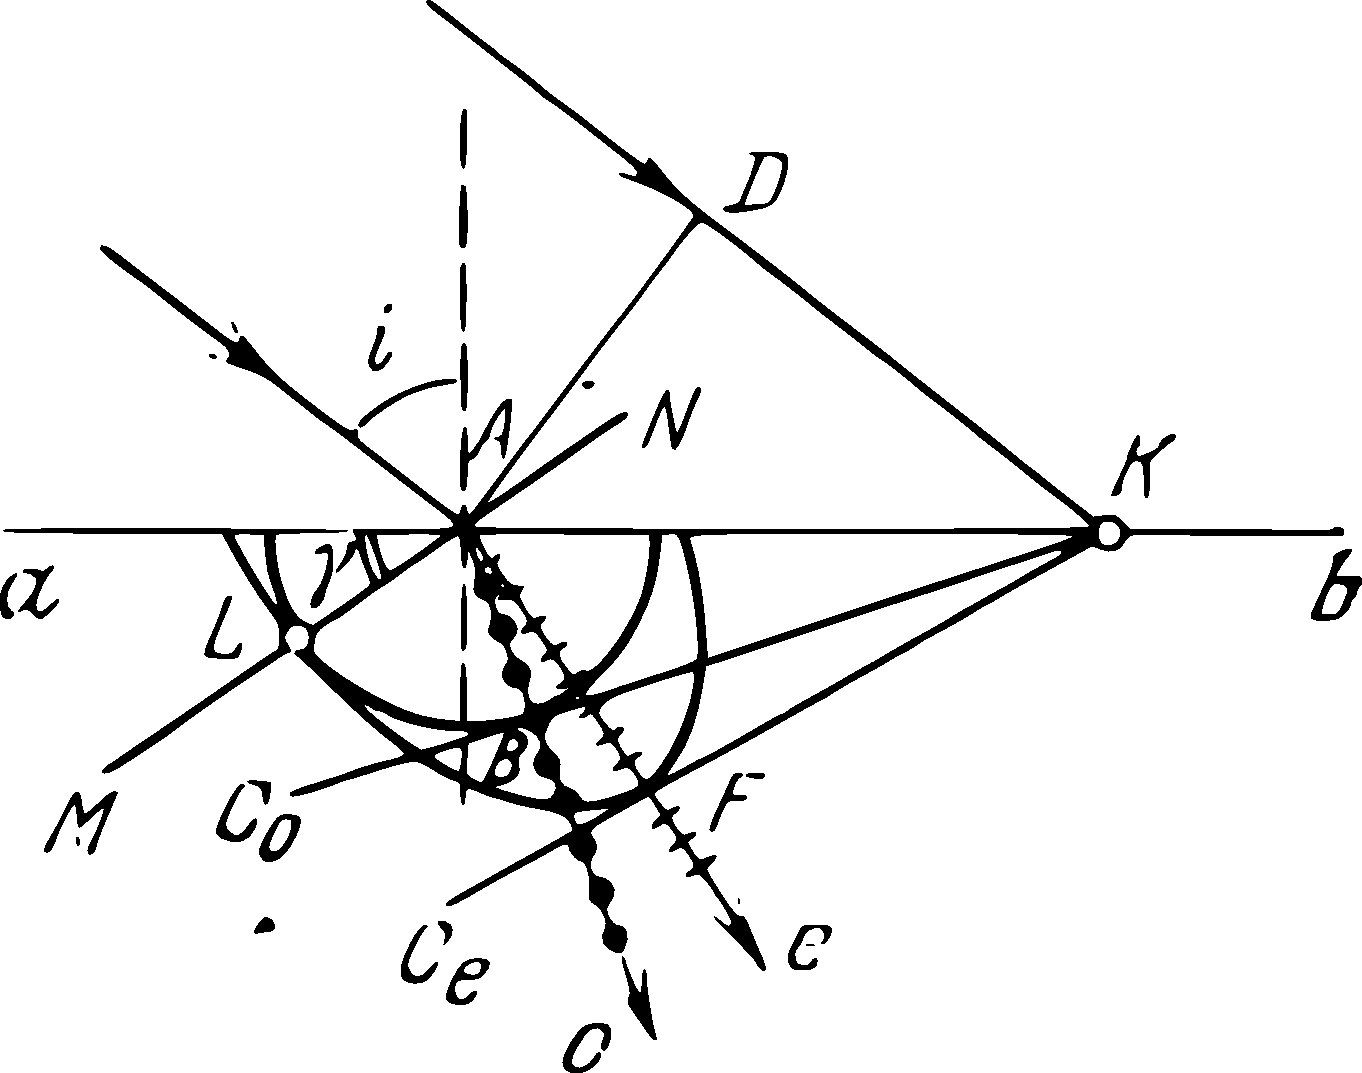
\includegraphics[width=\textwidth]{figs/ch-35/fig-35-06.pdf}
\sidecaption{Analysing birefringence in a uniaxial crystal using the Huygens graphical method.\zhcap{用惠更斯作图法分析单轴晶体中的双折射。}\label{fig-35-06}}
\end{marginfigure}


\subsection{}\label{35.2.6} The \redem{ray surface of a wave in a crystal} is the locus of the heads of vectors $\vb{v}$ of the ray velocity of the wave that extend from a certain point $O$ in the crystal in all possible directions. 
\zhpar{晶体中某一波的\redem{射线面}，是指从晶体中某点 $O$ 出发、沿一切可能方向画出的该波射线速度矢量 $\vb{v}$ 的末端所构成的轨迹。}



In a uniaxial crystal, the ray surface of the ordinary wave has the shape of a sphere, whereas that of the extraordinary wave is an ellipsoid of revolution about the optic axis $MN$ passing through point $O$. The ellipsoid and sphere contact each other at the points of intersection with optic axis $MN$. When $n_{e} \geqslant  n_{o}$, the ellipsoid is inscribed in the sphere (\figr{fig-35-05}~(a)), whereas if $n_{e} \leqslant  n_{o}$ the ellipsoid is circumscribed about the sphere (\figr{fig-35-05}~(b)). In the former case, the uniaxial crystal is said to be \redem{optically positive}, in the latter, \redem{optically negative}.
\zhpar{在单轴晶体中，寻常波的射线面为球面，而非常波的射线面是绕通过点 $O$ 的光轴 $MN$ 旋转的旋转椭球面。椭球面与球面在与光轴 $MN$ 的交点处相互接触。当 $n_{e} \geqslant n_{o}$ 时，椭球面内切于球面（\figr{fig-35-05}~(a)）；而当 $n_{e} \leqslant n_{o}$ 时，椭球面外切于球面（\figr{fig-35-05}~(b)）。前一种情形下，该单轴晶体称为\redem{光学正晶体}，后一种情形下称为\redem{光学负晶体}。}

\subsection{}\label{35.2.7} Birefringence in a uniaxial crystal can be explained and the directions of the ordinary and extraordinary rays can be found by using the Huygens graphical method. Assume that a plane unpolarized light wave is incident on the plane surface $ab$ of a uniaxial optically negative crystal (or a plate cut out of this crystal) at the angle $i$ (\figr{fig-35-06}). The optic axis $MN$ of the crystal, passing through point $A$ of surface $ab$, lies in
 the plane of the figure and makes the angle $\gamma$ with plane $ab$.
\zhpar{利用惠更斯作图法可以解释单轴晶体中的双折射，并求出寻常光线和非常光线的方向。设一平面非偏振光波以角度 $i$ 入射到光学负单轴晶体（或由该晶体切出的平板）的平面 $ab$ 上（见\figr{fig-35-06}）。晶体的光轴 $MN$ 经过表面 $ab$ 上的点 $A$，位于图面内，并与平面 $ab$ 成夹角 $\gamma$。}

At the instant $t$ of time being considered, the front $AD$ of the incident wave has reached pointed on the surface of the crystal, and this point becomes the source of two linearly polarized elementary secondary waves, ordinary and extraordinary, in the crystal. At the instant of time $t + \Delta t$, where $\Delta t$ is the time required for the incident light to travel the distance $\seg{DK}$, the
disturbance, propagating from point $A$ in the form of the ordinary elementary wave, reaches the points of a sphere of radius $v_{0}\Delta t$ having its centre at point $A$. 
\zhpar{在所考虑的时刻 $t$，入射波的波前 $AD$ 已到达晶体表面上的一点，该点成为晶体内寻常和非常两个线偏振次级子波的波源。在时刻 $t + \Delta t$（其中 $\Delta t$ 为入射光通过距离 $\seg{DK}$ 所需的时间）时，从点 $A$ 以寻常子波形式传播的扰动，到达以点 $A$ 为球心、半径为 $v_{0}\Delta t$ 的球面上各点。}

The disturbance, propagating from point $A$ in the form of the extraordinary elementary wave, reaches points at the same time on the surface of the ellipsoid of revolution that contacts the sphere of radius v0At at point $L$ of its intersection with optic axis $MN$. This ellipsoid is geometrically
similar to the ray surface of the extraordinary wave in
the crystal \ssect{35.2.5}. 
\zhpar{与此同时，从点 $A$ 以非常子波形式传播的扰动，到达一个旋转椭球面上的各点，该椭球面与上述半径为 $v_{0}\Delta t$ 的球面相切于其与光轴 $MN$ 的交点 $L$。该椭球面与晶体中非常波的射线面几何相似\ssect{35.2.5}。}

Planes $KC_{o}$ and $KC_{e}$, perpendicular to the plane of the figure and tangent, respectively, to the sphere and the ellipsoid, indicate, according to the Huygens principle \ssect{33.1.1}, the positions, at the instant of time $t + \Delta t$, of the fronts of the ordinary and extraordinary waves that actually propagate in a uniaxial crystal. Straight lines from point $A$ to the points of tangency $B$ and $F$ indicate the directions of the ordinary and extraordinary rays. Both rays lie in the plane of incidence, but the extraordinary ray is not orthogonal to the wave surface $KC_{e}$. 
\zhpar{根据惠更斯原理\ssect{33.1.1}，垂直于图面、且分别与球面和椭球面相切的平面 $KC_{o}$ 和 $KC_{e}$，给出了时刻 $t + \Delta t$ 时晶体中实际传播的寻常波和非常波波前的位置。从点 $A$ 到切点 $B$ 和 $F$ 的直线分别指示寻常光线和非常光线的方向。两条光线都位于入射面内，但非常光线与波面 $KC_{e}$ 并不正交。}

The ordinary and extraordinary waves are linearly polarized in mutually perpendicular planes. The directions of the electric vectors $\vb{E}_{o}$ and $\vb{E}_{e}$ in the ordinary and extraordinary waves are shown in \figr{fig-35-06} by black dots and transverse dashes located on the corresponding rays.
\zhpar{寻常波和非常波是在相互垂直的平面内线偏振的。寻常波与非常波中电矢量 $\vb{E}_{o}$ 和 $\vb{E}_{e}$ 的方向，在\figr{fig-35-06}中分别以位于相应光线上的黑点和短横线表示。}


\begin{figure}%[-3cm] 
\centering
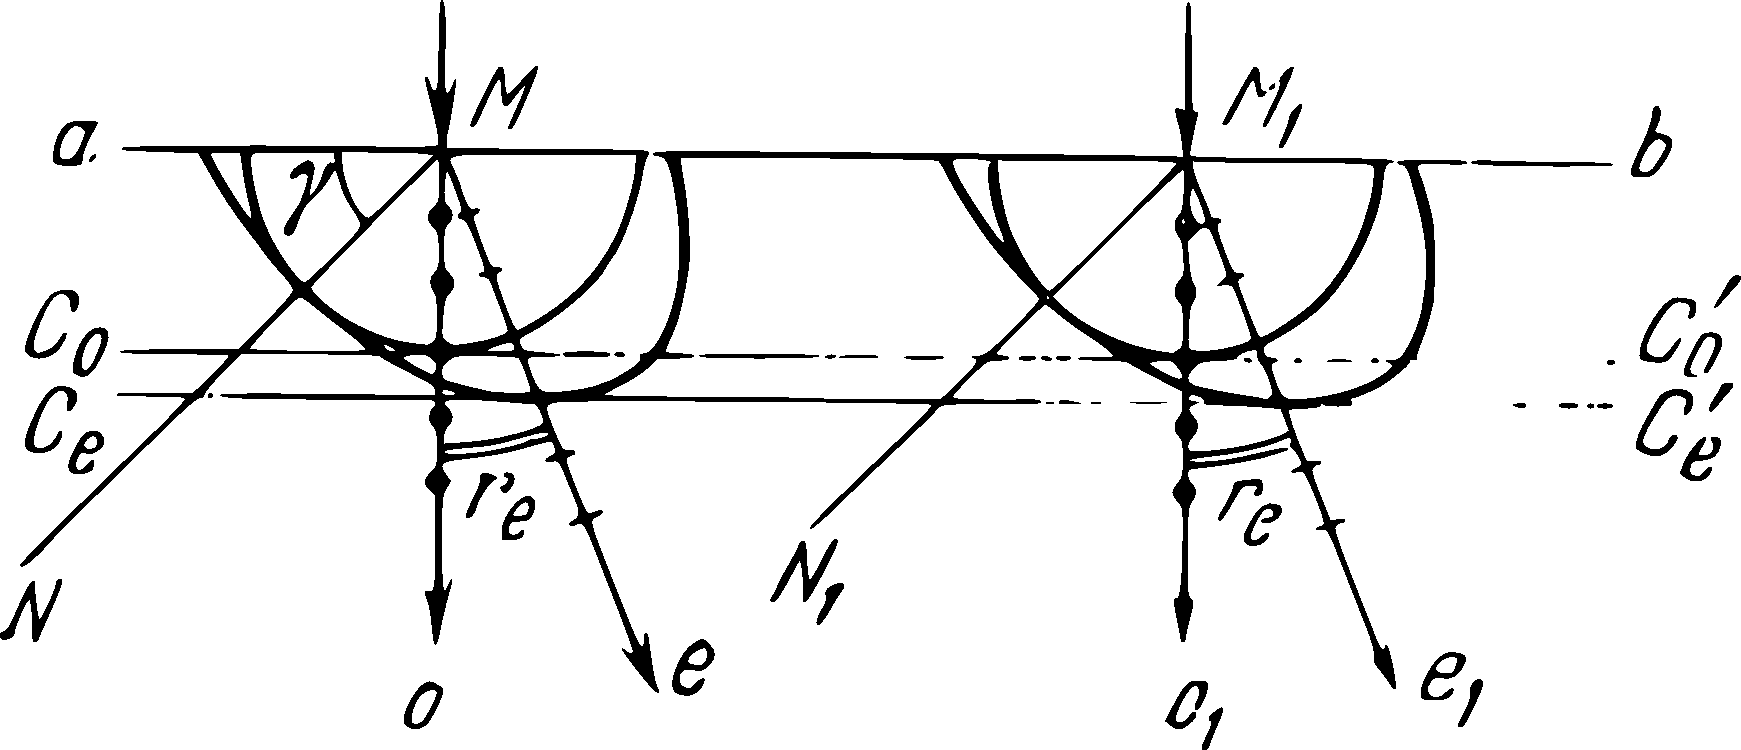
\includegraphics[width=\textwidth]{figs/ch-35/fig-35-07.pdf}
\sidecaption{The ordinary and extraordinary rays in the case of normal incidence of light on the surface of
an optically negative uniaxial crystal.\zhcap{光垂直入射到光学负单轴晶体表面时的寻常光线与非常光线。}\label{fig-35-07}}
\end{figure}

\hlblue{Note.} If the optic axis $MN$ of the crystal does not lie in the plane of incidence of the light, then, in general, the extraordinary ray also does not lie in the plane of incidence. Consequently, the angle between the planes of polarization of the ordinary and extraordinary waves differs slightly from a right angle.
\zhpar{\hlblue{注意：}若晶体光轴 $MN$ 不位于光的入射面内，则一般而言非常光线也不位于入射面内。因此，寻常波与非常波偏振面之间的夹角与直角略有偏差。}



\subsection{}\label{35.2.8}. The construction for the ordinary and extraordinary rays in the case of normal incidence of light on the surface of an optically negative uniaxial crystal is shown in \figr{fig-35-07}. Here $ab$ is the position of the incident wavefront at the instant $t$ of time, and $C_{o}C_{o}'$ and $C_{e}C_{e}'$ are the positions of the fronts of the ordinary and extraordinary waves in the crystal at the instant of time $t + \Delta t$.
\zhpar{光垂直入射到光学负单轴晶体表面时，寻常光线与非常光线的作图如\figr{fig-35-07}所示。其中 $ab$ 为时刻 $t$ 入射波前的位置，$C_{o}C_{o}'$ 和 $C_{e}C_{e}'$ 分别为时刻 $t + \Delta t$ 时晶体中寻常波和非常波波前的位置。}
\begin{marginfigure}%[-3cm] 
\centering
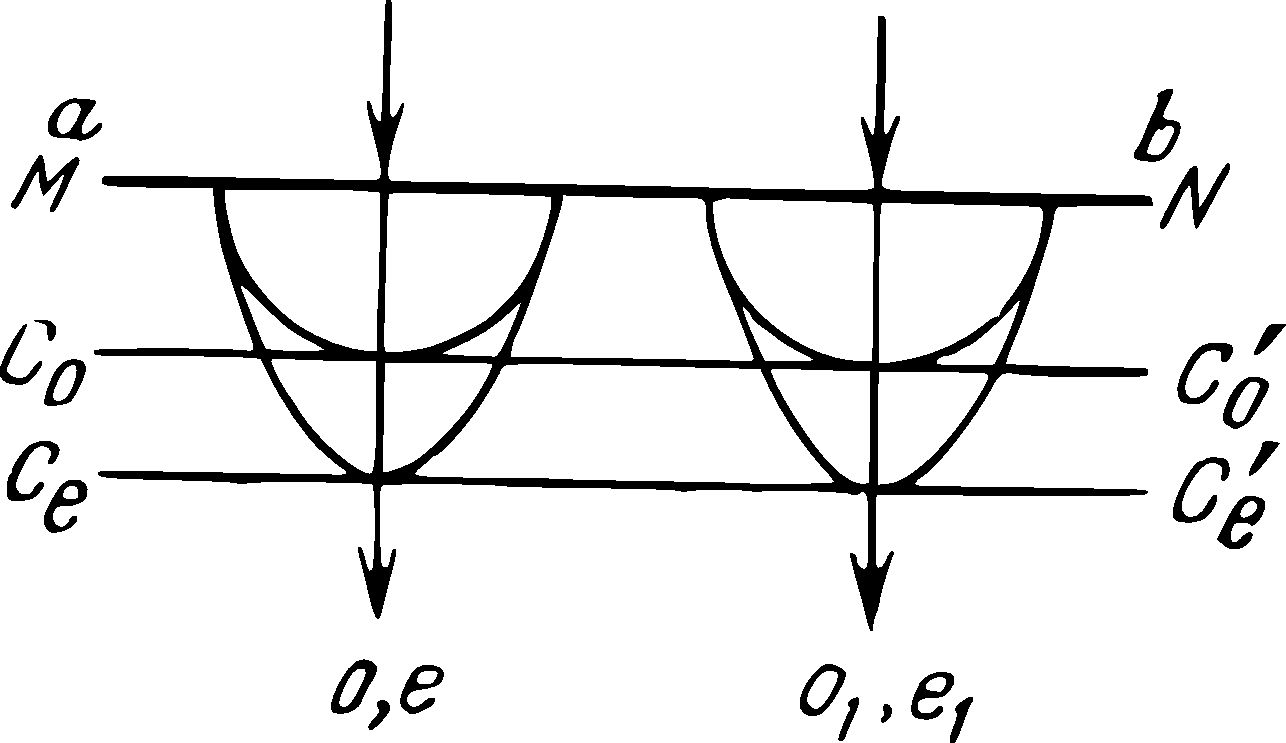
\includegraphics[width=\textwidth]{figs/ch-35/fig-35-08.pdf}
\sidecaption{Analysing the case when light is normally
incident on the plane surface of an optically negative uniaxial crystal.\zhcap{分析光垂直入射到光学负单轴晶体平面上的情形。}\label{fig-35-08}}
\end{marginfigure}


It is assumed that the optic axis $M$N lies in the plane of incidence and makes the angle $\gamma$, differing from 0 and $\pi/2$, with the refracting surface $ab$. It is evident from \figr{fig-35-07} that the ordinary ray is an extension of the incident one and that the extraordinary ray is refracted
by the angle $r_{e} \neq 0$.
\zhpar{设光轴 $MN$ 位于入射面内，并与折射面 $ab$ 成不等于 $0$ 和 $\pi/2$ 的夹角 $\gamma$。由\figr{fig-35-07}可以看出，寻常光线是入射光线的延长线，而非常光线发生折射，折射角 $r_{e} \neq 0$。}



Considered in \figr{fig-35-08} is a case in which light is normally incident on the plane surface $ab$ of an optically negative uniaxial crystal, whose optic axis $MN$ is parallel to $ab$. Here, as is evident from the construction, the extraordinary ray is not refracted at the surface ab and
coincides in direction with the ordinary and incident
rays. But the velocities of the ordinary and extraordinary
rays in the crystal in this direction differ and are respectively equal to \ssect{35.2.5}: $v_{o} = c/n_{o}$ and $v_{e} = c/n_{eo}$. Therefore, the two rays  (waves) travel the same distance $d$ in the crystal with an optical-path difference \ssect{32.3.2}: 
\zhpar{如\figr{fig-35-08}所示，光垂直入射到光学负单轴晶体的平面 $ab$ 上，且其光轴 $MN$ 与 $ab$ 平行。由作图可见，非常光线在表面 $ab$ 处不发生折射，其方向与寻常光线和入射光线一致。但在这一方向上，寻常光线与非常光线在晶体中的速度不同，分别为\ssect{35.2.5}：$v_{o} = c/n_{o}$ 和 $v_{e} = c/n_{eo}$。因此，两束光线（波）在晶体中经过相同距离 $d$ 时存在光程差\ssect{32.3.2}：}
\begin{equation*}%
\Delta s = d (n_{o} - n_{eo}).
\end{equation*}


\subsection{}\label{35.2.9} The path of the rays in a \redem{polarizing prism} are shown in \figr{fig-35-09}. This prism is cut out of a crystal of Iceland spar so that its sides $AB$ and $CD$ are parallel to its optic axis $MN$. Then the prism is cut apart along its diagonal plane $AC$ and
glued together along these diagonal surfaces by a thin layer of an optically isotropic transparent substance called Canada balsam.
\zhpar{偏振棱镜中光线的路径如\figr{fig-35-09}所示。该棱镜由冰洲石晶体切割而成，使其侧面 $AB$ 和 $CD$ 与晶体光轴 $MN$ 平行。然后沿其对角面 $AC$ 将棱镜切开，并用一薄层光学各向同性的透明物质——加拿大树胶沿这些对角面重新胶合起来。}
\begin{marginfigure}%[-3cm] 
\centering
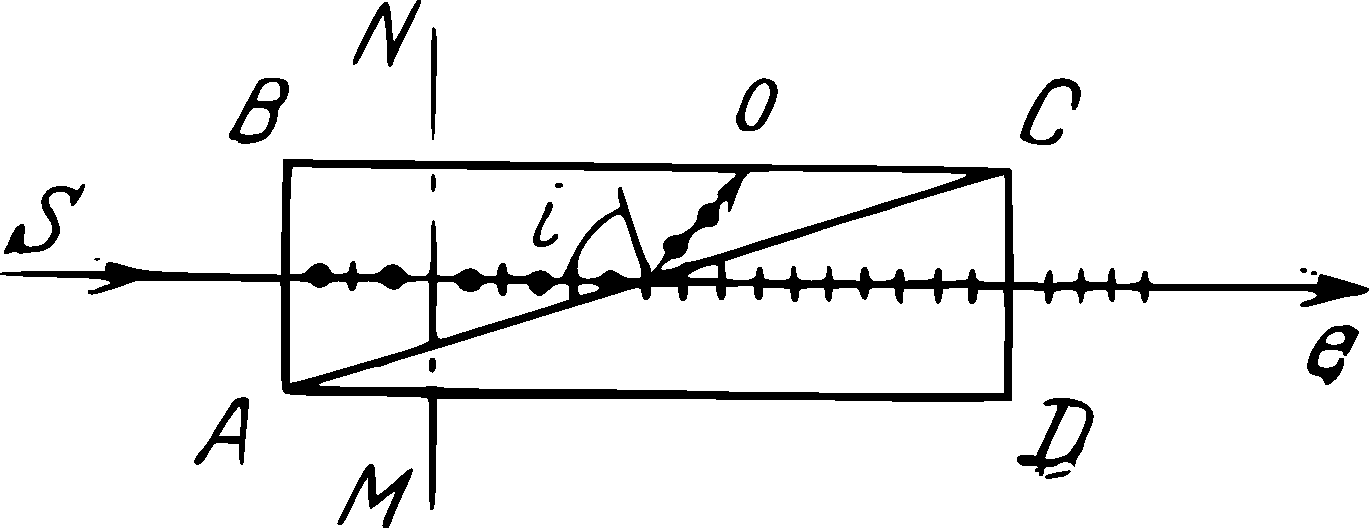
\includegraphics[width=\textwidth]{figs/ch-35/fig-35-09.pdf}
\sidecaption{The path of rays in a polarising prism.\zhcap{偏振棱镜中光线的路径。}\label{fig-35-09}}
\end{marginfigure}

The crystal of Iceland spar is uniaxial and optically negative; its refractive indices \ssect{35.2.5} are: $n_{o} = 1.658 $ and $n_{eo} = 1.486$. The refractive index of Canada balsam is $n_{Cb} = 1.550$, i.e. Canada balsam is a medium less optically dense than the material of the prism for the ordinary ray and more optically dense than this material for the extraordinary ray. Light falls on the prism normal to its side $AB$ (ray $S$ in \figr{fig-35-09}). 
\zhpar{冰洲石是单轴光学负晶体，其折射率\ssect{35.2.5}为 $n_{o} = 1.658$，$n_{eo} = 1.486$。加拿大树胶的折射率为 $n_{Cb} = 1.550$，即对寻常光线而言，加拿大树胶是比棱镜材料光密程度小的介质，而对非常光线而言，它则是比棱镜材料光密程度大的介质。光沿法线方向射到棱镜的侧面 $AB$ 上（见\figr{fig-35-09}中的光线 $S$）。}

The ordinary and extraordinary rays propagate in the prism without being refracted until they reach the layer $AC$ of Canada balsam. The dimensions of the prism are selected so that the angle of incidence $i$ of the ordinary ray on surface $AC$ is greater than the critical angle for total internal reflection \ssect{31.5.8}. Therefore, the ordinary wave is completely reflected by the layer of Canada balsam (ray $o$ in \figr{fig-35-09}). The extraordinary wave passes freely through the layer of Canada balsam and the second half of the polarizing prism. Thus, the polarizing prism can be used as a
polarizer \ssect{35.1.2}.
\zhpar{寻常光线和非常光线在棱镜中传播时都不发生折射，直至到达加拿大树胶层 $AC$。棱镜的尺寸经过选择，使寻常光线在面 $AC$ 上的入射角 $i$ 大于全内反射的临界角\ssect{31.5.8}。因此，寻常光被加拿大树胶层全反射（见\figr{fig-35-09}中的光线 $o$）。非常光则可以自由地穿过加拿大树胶层和棱镜的另一半。这样，偏振棱镜便可用作起偏器\ssect{35.1.2}。}

\subsection{}\label{35.2.10} All birefringent crystals absorb light to one or another degree. This absorption is anisotropic: the absorption factor \ssect{34.2.1} depends upon the orientation of the electric vector of the light wave and on the direction of light propagation in the crystal, as well as on the wavelength. This phenomenon is called \redem{dichroism}, or \redem{pleochroism}, because it is manifested in the different colouring of the crystals in different directions. An example of a strongly dichroic crystal is tourmaline, a uniaxial crystal in which the ordinary ray is absorbed much more intensely than the extraordinary ray. Even more pronounced dichroism is displayed by crystals of herapathite, which is used to make thin films, converting natural light into linearly polarized light and called \redem{polaraids}.
\zhpar{所有双折射晶体都或多或少地吸收光。这种吸收是各向异性的：吸收因子\ssect{34.2.1}取决于光波电矢量的方向、光在晶体中的传播方向以及光的波长。这种现象称为\redem{二色性}，或\redem{多色性}，因为它表现为晶体在不同方向上呈现出不同的颜色。电气石是强二色性晶体的一个例子，它是单轴晶体，其中寻常光线的吸收远比非常光线强烈。赫拉帕石晶体的二色性更为显著，它常用于制作能将自然光转变为线偏振光的薄膜，这种薄膜称为\redem{偏振片}。}

\section{Interference of Polarized Light}
\label{sec-35.3} 
\zhtitle{偏振光的干涉}


\subsection{}\label{35.3.1} Trains of waves with all possible orientations with respect to the ray of their planes of polarization, included in the composition of natural light, are incoherent because they correspond to the radiation of various \redem{independent} atoms of the light source. All these trains participate in the formation of the ordinary and extraordinary waves that propagate in a uniaxial crystal when natural light falls on it. 
\zhpar{构成自然光的各波列，其偏振面相对于光线具有各种可能的取向，它们彼此不相干，因为它们分别对应于光源中各个独立原子的辐射。当自然光射到单轴晶体上时，所有这些波列都参与了晶体中寻常波和非常波的形成。}

But the contribution of each separate train to these two waves is, in general, not the same. It is greater to the wave whose plane of polarization makes the smaller angle a with the plane of polarization of the wave train. In other words, the ordinary and extraordinary waves are generated mainly by \redem{different} wave trains included in the composition of natural light. Consequently, the ordinary and extraordinary waves, propagated in a uniaxial crystal on which natural light falls, are not coherent.
\zhpar{但是，各个波列对这两种波的贡献一般并不相同：偏振面与该波列偏振面的夹角 $\alpha$ 较小的那一种波，所得到的贡献较大。换言之，寻常波和非常波主要是由构成自然光的\redem{不同}波列产生的。因此，自然光入射到单轴晶体后，在晶体中传播的寻常波和非常波是不相干的。}
\begin{marginfigure}[-1cm] 
\centering
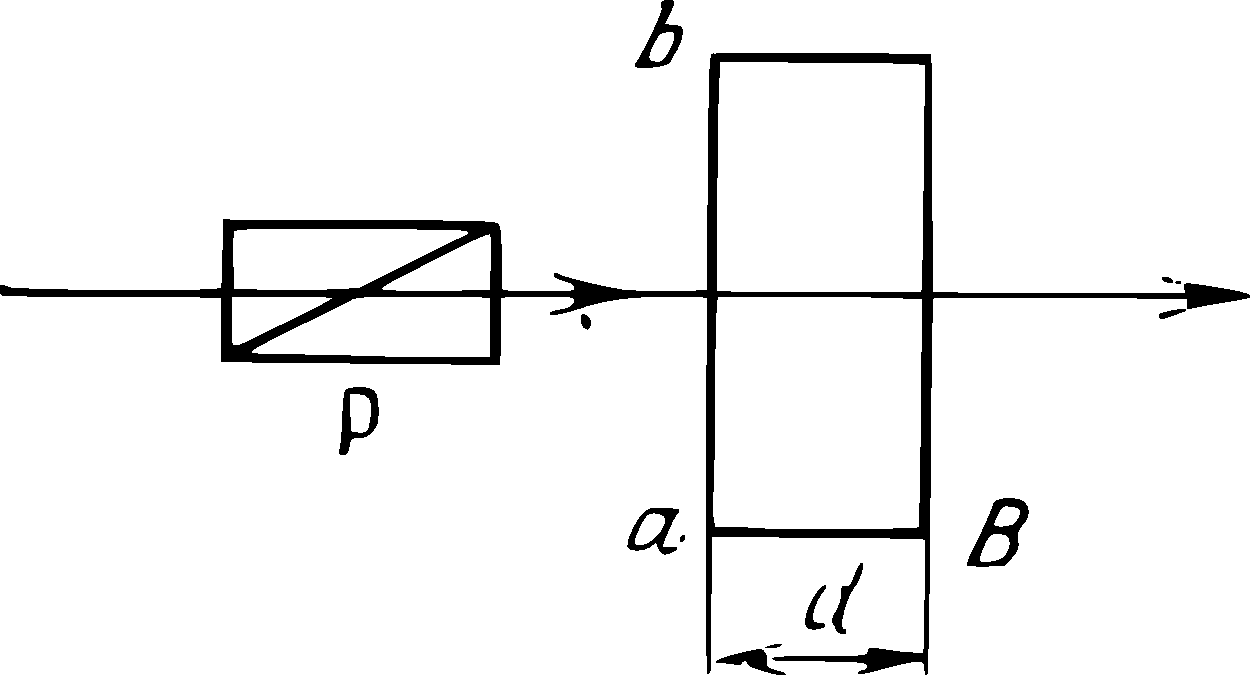
\includegraphics[width=\textwidth]{figs/ch-35/fig-35-10.pdf}
\sidecaption{Analysing beams passing through a polariser.\zhcap{分析通过起偏器的光束。}\label{fig-35-10}}
\end{marginfigure}
\subsection{}\label{35.3.2} The ordinary and extraordinary waves, propagated in a uniaxial crystal upon the incidence of linearly polarized light [obtained from natural light by means, for example, of a polarizing prism \ssect{35.2.9} or some other polarizer] are coherent with each other. This is due to the fact that the planes of polarization of all the wave trains included in the composition of the incident light have the same orientation.
\zhpar{当线偏振光〔例如借助偏振棱镜\ssect{35.2.9}或其他起偏器由自然光获得〕入射到单轴晶体上时，在晶体中传播的寻常波和非常波是彼此相干的。这是因为入射光中所有波列的偏振面都具有相同的取向。}



\begin{marginfigure}%[-3cm] 
\centering
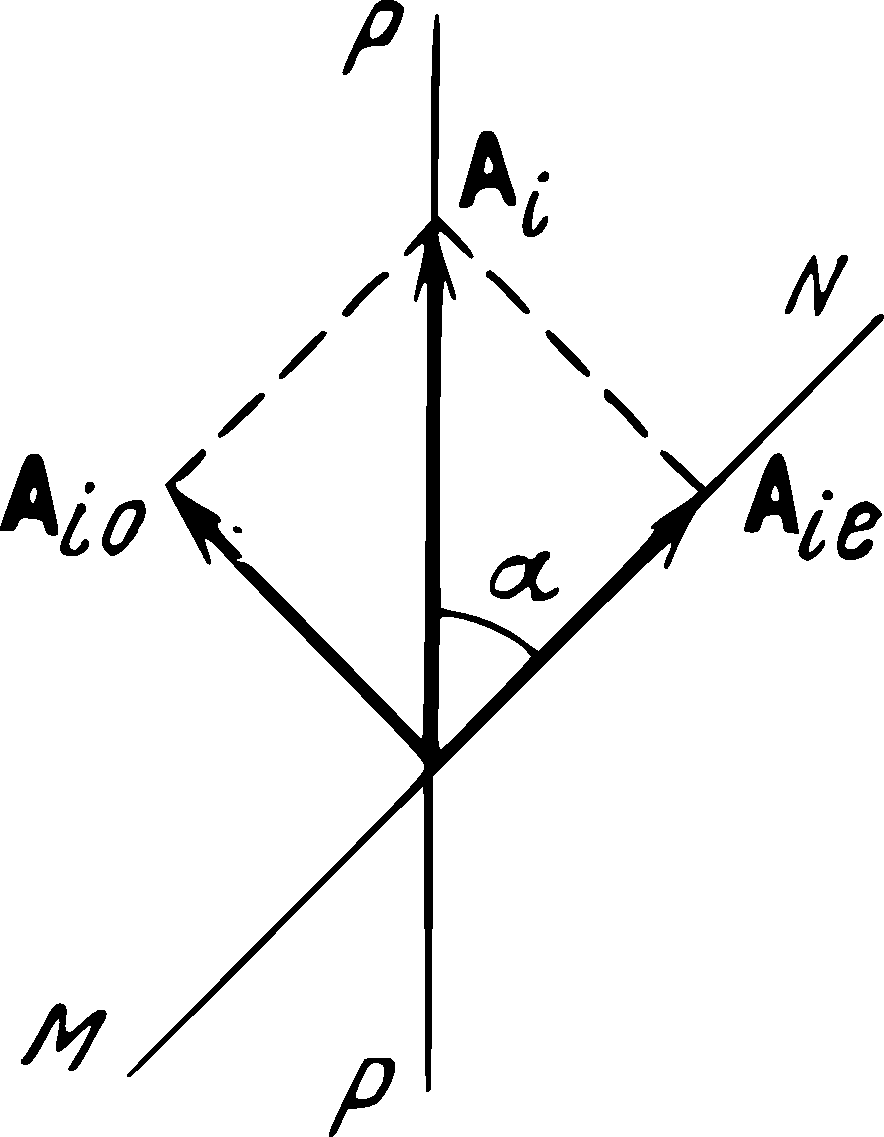
\includegraphics[width=0.7\textwidth]{figs/ch-35/fig-35-11.pdf}
\sidecaption{Analysing beams passing through a polariser.\zhcap{分析通过起偏器的光束。}\label{fig-35-11}}
\end{marginfigure}

Assume that a parallel beam of light, after passing through polarizer $P$ (\figr{fig-35-10}), is normally incident on the plane surface $ab$ of plane-parallel plate $B$, cut out of a uniaxial crystal parallel to its optic axis $MN$ (axis $MN$ is parallel to plane $ab$). Shown in \figr{fig-35-11} is vector $\vb{A}_{i}$ of the amplitude of the $i$-th wave train.
\zhpar{设一束平行光经过起偏器 $P$（见\figr{fig-35-10}）后，垂直入射到由单轴晶体切割而成、光轴 $MN$ 平行于平面 $ab$ 的平行平板 $B$ 的平面 $ab$ 上。\figr{fig-35-11}中给出了第 $i$ 个波列振幅矢量 $\vb{A}_{i}$。}



This vector is oriented along line $p-p$, corresponding to the direction of oscillation of the electric vector in the light emerging from the polarizer. The contributions of the ith wave train to the ordinary and extraordinary waves are characterized by the amplitudes $A_{io} = A_{i} \sin \alpha$ and $A_{ie} - A_{i} = \cos \alpha$, whose ratio
$A_{io}/A_{ie} = \tan \alpha$ is the same for all trains. In particular, if $\alpha = \pi/4$, then $A_{io} = A_{ie}$ because pairwise coherent trains, polarized in mutually perpendicular planes, have the same intensity.
\zhpar{该矢量沿直线 $p$-$p$ 方向，对应于从起偏器射出的光中电矢量的振动方向。第 $i$ 个波列对寻常波和非常波的贡献分别由振幅 $A_{io} = A_{i} \sin \alpha$ 和 $A_{ie} - A_{i} = \cos \alpha$ 表征，它们之比 $A_{io}/A_{ie} = \tan \alpha$ 对所有波列都相同。特别地，若 $\alpha = \pi/4$，则 $A_{io} = A_{ie}$，因为偏振面相互垂直的成对相干波列具有相同的强度。}

\subsection{}\label{35.3.3} At the entrance to crystal plate $B$ \ssect{35.3.2}, the electric vectors $\vb{E}_{0}$ and $\vb{E}_{e}$ of the ordinary and extraordinary waves oscillate
in phase and their vector sum is equal to electric vector
of linearly polarized monochromatic incident light: $\vb{E}_{p} = \vb{E}_{0} + \vb{E}e$. In the plate the ordinary and extraordinary waves propagate at different velocities \ssect{35.2.8}. Therefore, at the exit from the plate (of thickness $d$), the mutually perpendicular electric
vectors $\vb{E}_{o}'$ and $\vb{E}_{e}'$ of the ordinary and extraordinary waves oscillate with a phase difference of
\zhpar{在进入晶片 $B$ 处\ssect{35.3.2}，寻常波和非常波的电矢量 $\vb{E}_{0}$ 与 $\vb{E}_{e}$ 同相振动，二者的矢量和等于入射的线偏振单色光的电矢量：$\vb{E}_{p} = \vb{E}_{0} + \vb{E}e$。由于寻常波与非常波在晶片中以不同速度传播\ssect{35.2.8}，因此从厚度为 $d$ 的晶片射出时，相互垂直的寻常波电矢量 $\vb{E}_{o}'$ 与非常波电矢量 $\vb{E}_{e}'$ 之间的相位差为}
\begin{equation*}%
\Delta \varphi = \frac{2 \pi \Delta s}{\lambda_{0}} =\frac{2 \pi d}{\lambda_{0}} (n_{0} - n_{eo})
\end{equation*}
where $ \Delta s$ is the optical-path difference of these waves \ssect{35.2.8}, and $\lambda_{0}$ is the wavelength of light in vacuum. Consequently, as a result of its passing through the plate, the light, in the general case, becomes elliptically polarized \ssect{31.1.7}: the head of vector
$\vb{E}' = \vb{E}'_{o} + \vb{E}_{e}'$ describes an ellipse lying in a plane perpendicular to the beam. If $\alpha$ is the angle between the direction of oscillation of vector $\vb{E}_{p}$ and the optic axis $MN$ of the plate, then amplitudes ${A}_{o}$ and ${A}_{e}$ of vectors $\vb{E}_{o}$ and $\vb{E}_{e}$ equal: $A_{o} = Ap \sin \alpha$ and $A_{e} = Ap \cos \alpha$, where $A_{p}$ is the amplitude of vector $\vb{E}_{p}$.
\zhpar{式中 $\Delta s$ 为这两个波的光程差\ssect{35.2.8}，$\lambda_{0}$ 为真空中光的波长。因此，光通过晶片后一般变为椭圆偏振光\ssect{31.1.7}：矢量 $\vb{E}' = \vb{E}'_{o} + \vb{E}_{e}'$ 的末端描绘出位于垂直于光束的平面内的一个椭圆。若 $\alpha$ 为矢量 $\vb{E}_{p}$ 的振动方向与晶片光轴 $MN$ 之间的夹角，则矢量 $\vb{E}_{o}$ 与 $\vb{E}_{e}$ 的振幅分别为 $A_{o} = Ap \sin \alpha$ 和 $A_{e} = Ap \cos \alpha$，式中 $A_{p}$ 为矢量 $\vb{E}_{p}$ 的振幅。}

In the absence of light absorption in the plate, the amplitudes of vectors $\vb{E}'_{o}$ and $\vb{E}'_{e}$ are also equal to $A_{o}$ and $A_{e}$.
\zhpar{若光在晶片中无吸收，则矢量 $\vb{E}'_{o}$ 与 $\vb{E}'_{e}$ 的振幅也分别等于 $A_{o}$ 和 $A_{e}$。}

\subsection{}\label{35.3.4} In accordance with the thickness $d$ of the plate, several special cases are possible.
\zhpar{根据晶片厚度 $d$ 的不同，可能出现以下几种特殊情形：}
\begin{enumerate}[label=(\alph*)]
\item A \redem{quarter-wave plate} is one whose thickness satisfies the relation: $d(n_{o} - n_{eo}) = \pm (m + 1/4) \lambda_{0}$, where $m = 0, \,1,\, 2, \ldots{}$; the plus sign corresponding to an optically negative crystal, and the minus sign to an optically positive one \ssect{35.2.6}. At the
exit from such a plate the oscillations of vectors $\vb{E}_{o}'$ and $\vb{E}_{e}'$ have a phase difference of $\pi/2$. If, in addition, $\alpha = \pi/4$, the light emerging from the plate is circularly polarized \ssect{31.1.7}.
\zhpar{\redem{四分之一波片}是指厚度满足下列关系的晶片：$d(n_{o} - n_{eo}) = \pm (m + 1/4) \lambda_{0}$，式中 $m = 0,\, 1,\, 2, \ldots{}$；其中正号对应于光学负晶体，负号对应于光学正晶体\ssect{35.2.6}。光从这种晶片射出时，矢量 $\vb{E}_{o}'$ 与 $\vb{E}_{e}'$ 的振动之间的相位差为 $\pi/2$。若此外还有 $\alpha = \pi/4$，则从晶片射出的光为圆偏振光\ssect{31.1.7}。}
\begin{marginfigure}%[-3cm] 
\centering
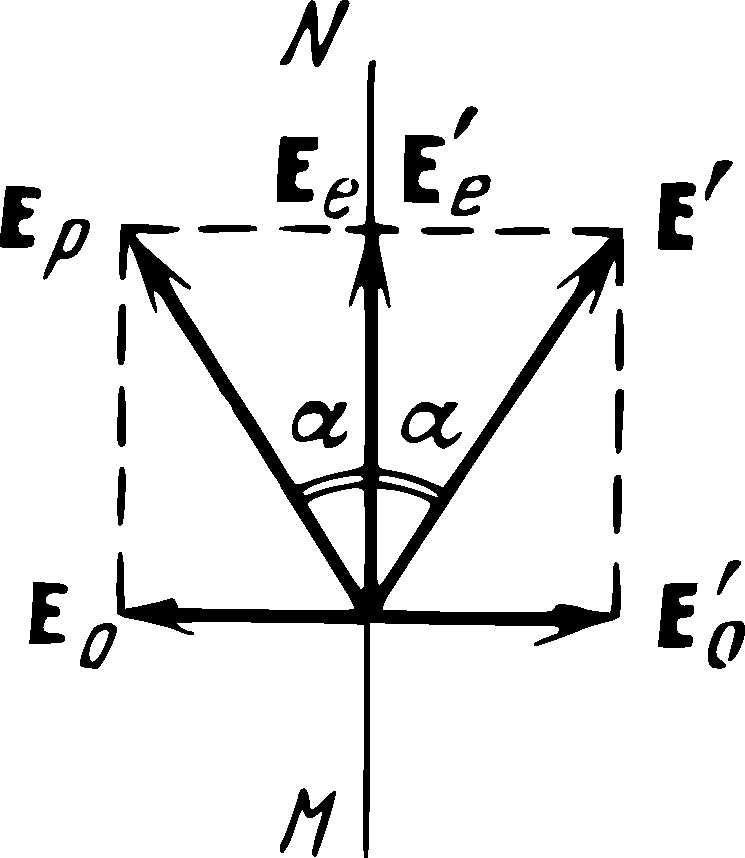
\includegraphics[width=0.7\textwidth]{figs/ch-35/fig-35-12.pdf}
\sidecaption{Half-wave plate.\zhcap{半波片。}\label{fig-35-12}}
\end{marginfigure}

\item For a \redem{half-wave plate}: $d (n_{o} - n_{eo}) = \pm (m + 1/2) \lambda_{0}$. At the exit from such a plate, the oscillations of vectors $\vb{E}_{o}'$ and $\vb{e}'$ have a phase difference of $\pi$. Light emerging from the
plate remains linearly polarized. But the directions of oscillation of vectors $\vb{E}_{p}$ and $\vb{E}'$ of the incident and transmitted light are symmetrical with respect to the principal plane of the plate (\figr{fig-35-12}).
\zhpar{\redem{半波片}：$d (n_{o} - n_{eo}) = \pm (m + 1/2) \lambda_{0}$。光从这种晶片射出时，矢量 $\vb{E}_{o}'$ 与 $\vb{e}'$ 的振动之间的相位差为 $\pi$。从晶片射出的光仍为线偏振光，但入射光与透射光的电矢量 $\vb{E}_{p}$ 与 $\vb{E}'$ 的振动方向相对于晶片主平面是对称的（见\figr{fig-35-12}）。}

\item For a \redem{full-wave plate}: $d (n_{o} - n_{eo}) = \pm m \lambda_{0}$ a result of passing through the plate, the light remains linearly polarized in the same plane as the incident light.
\zhpar{\redem{全波片}：$d (n_{o} - n_{eo}) = \pm m \lambda_{0}$。光通过晶片后，仍保持线偏振，且偏振面与入射光的偏振面位于同一平面内。}
\end{enumerate}

\subsection{}\label{35.3.5} Coherent waves emerging from
crystal plate $B$ (\figr{fig-35-10}) cannot display interference because they are polarized in mutually perpendicular planes. Therefore, one more polarizing prism, the analyzer $A$ (\figr{fig-35-13}) is mounted beyond plate $B$. The analyzer
separates out of the incident coherent waves, the components polarized in one plane. It thus provides the conditions necessary for obtaining the interference of these waves. The results of this interference depend upon the phase difference
$\Delta \varphi$ acquired by the ordinary and extraordinary waves in the plate, on the ratio of the amplitudes of these waves and on the angle $\beta$ between the principal planes of the analyzer and polarizer \ssect{35.1.2}.
\zhpar{从晶片 $B$ 射出的相干波（见\figr{fig-35-10}）由于偏振面相互垂直，不能产生干涉。因此，在晶片 $B$ 之后再安装一个偏振棱镜，即检偏器 $A$（见\figr{fig-35-13}）。检偏器从入射的相干波中分离出沿同一平面偏振的分量，从而提供了这些波发生干涉所必需的条件。干涉结果取决于晶片中寻常波与非常波获得的相位差 $\Delta \varphi$、两波的振幅比，以及检偏器与起偏器主平面之间的夹角 $\beta$\ssect{35.1.2}。}

\begin{figure}%[-3cm] 
\centering
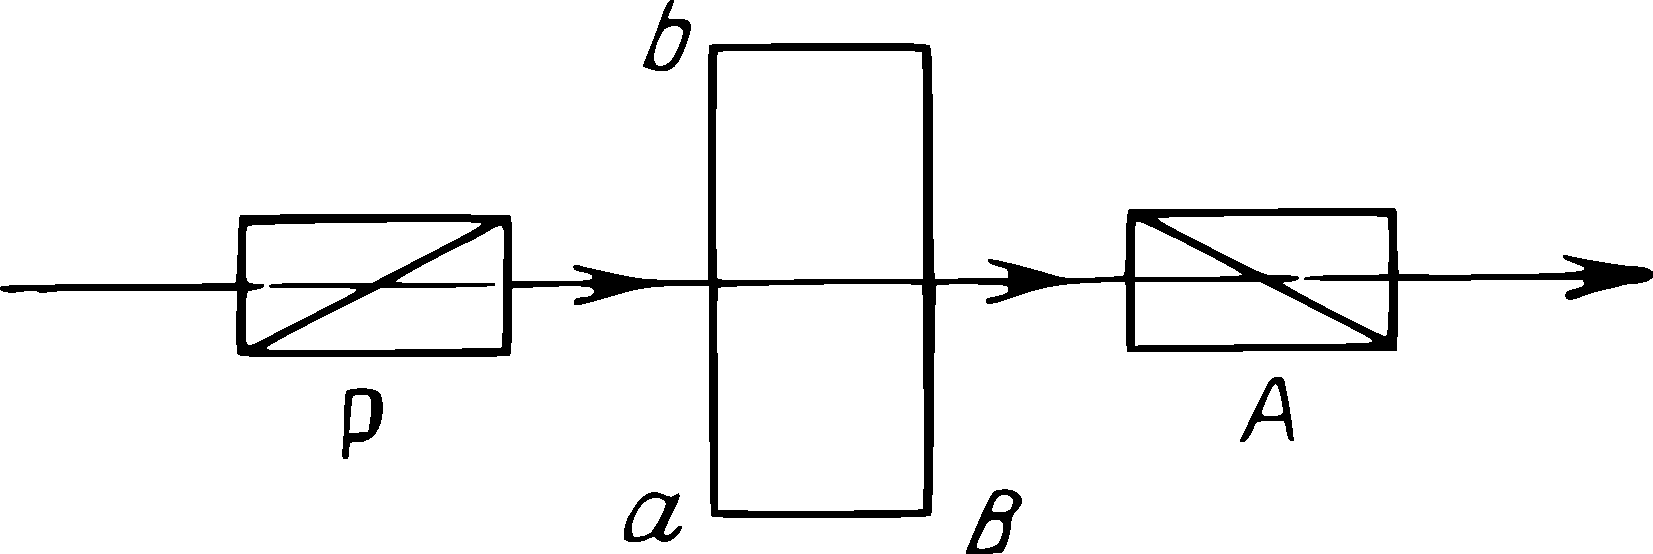
\includegraphics[width=0.7\textwidth]{figs/ch-35/fig-35-13.pdf}
\sidecaption{Making interference possible in coherent waves emerging from crystal plate.\zhcap{使从晶片射出的相干波能够发生干涉。}\label{fig-35-13}}
\end{figure}

For example, if the angle between the principal plane of the
polarizer and optic axis $MN$ of the plate $\alpha = \pi/4$, the amplitudes and intensities of the ordinary and extraordinary waves are the same. Assume in this case that monochromatic light of the wavelength $\lambda_{0}$ in vacuum is incident on the plate. The two following limiting cases may occur:
\zhpar{例如，若起偏器的主平面与晶片光轴 $MN$ 之间的夹角 $\alpha = \pi/4$，则寻常波与非常波的振幅和强度相等。设真空中波长为 $\lambda_{0}$ 的单色光射到晶片上。此时可能出现以下两种极限情形：}
\begin{equation*}%
\Delta \varphi = \frac{2\pi d}{\lambda_{0}}\, (n_{o} - n_{eo})) =  
\begin{cases}
\pm 2 m \pi \\
 \pm (2m +1)\pi,
\end{cases}
\end{equation*}
(where $m = 0,\, 1,\, 2,\, \ldots{})$.
In the first case, corresponding to a full-wave plate, the light falling on the analyzer is linearly polarized in the principal plane of the polarizer. Therefore, at $\beta = 0$ (the analyzer is mounted parallel to the polarizer), the intensity $I_{a}$ of the light passing through the analyzer is maximal, whereas at $\beta = \pi/2$ (the analyzer and polarizer are crossed), $I_{a} = 0$, i.e. at $\beta = 0$
an interference maximum is observed, whereas at $\beta = \pi/2 $ a minimum is observed.
\zhpar{（式中 $m = 0,\, 1,\, 2,\, \ldots{}$）。第一种情形对应于全波片，射到检偏器上的光为在起偏器主平面内的线偏振光。因此，当 $\beta = 0$（检偏器与起偏器平行放置）时，透过检偏器的光强 $I_{a}$ 最大；而当 $\beta = \pi/2$（检偏器与起偏器正交放置）时，$I_{a} = 0$。即在 $\beta = 0$ 时观察到干涉极大，而在 $\beta = \pi/2$ 时观察到干涉极小。}

In the second case, corresponding to a half-wave plate, the light falling on the analyzer is linearly polarized in a plane making the angle $2\alpha = \pi/2$ with the principal plane of the polarizer. Therefore, at $\beta = 0$ an interference minimum is observed, whereas at $\beta = \pi/2$ a maximum is observed.
\zhpar{第二种情形对应于半波片，射到检偏器上的光为线偏振光，其偏振面与起偏器主平面的夹角为 $2\alpha = \pi/2$。因此，当 $\beta = 0$ 时观察到干涉极小，而当 $\beta = \pi/2$ 时观察到干涉极大。}

If linearly polarized \redem{white light} is incident on plate $B$ (\figr{fig-35-13}), then in observing the light through the analyzer, the plate is seen to be coloured. Upon rotating the analyzer about the beam, i.e. in varying angle $\beta$, the colouring changes. This is due to the fact that the value of the phase difference $\Delta \varphi$, determining the result of interference, depends upon the wavelength of the light. 
\zhpar{若将线偏振的\redem{白光}射到晶片 $B$ 上（见\figr{fig-35-13}），则透过检偏器观察时，晶片呈现颜色。当绕光束转动检偏器，即改变角度 $\beta$ 时，颜色随之改变。这是因为决定干涉结果的相位差 $\Delta \varphi$ 的数值与光的波长有关。}

A plate, whose thickness $d$ is not the same at various
places, is seen in white light to be oddly coloured, with each coloured interference line (\redem{isochromate}) passing through points of equal thickness $d$. A similar pattern is observed in a plate, which is of equal thickness at all points, but the value of the difference
$(n_{o} - n_{eo})$ varies. In this case, each isochromatc passes through points of the plate corresponding to the same value of $(n_{o} - n_{eo})$.
\zhpar{厚度 $d$ 在各处不同的晶片，在白光中观察时呈现奇特的彩色条纹，每一条彩色干涉线（\redem{等色线}）都通过厚度相同的各点。对于各处厚度相同、但 $(n_{o} - n_{eo})$ 的值各处不同的晶片，也能观察到类似的图样。这时，每一条等色线通过晶片上 $(n_{o} - n_{eo})$ 值相同的各点。}

\section{ Artificial Optical Anisotropy}
\label{sec-35.4}
\zhtitle{人工光学各向异性}

\subsection{}\label{35.4.1} An optically isotropic transparent body becomes anisotropic if it is subjected to mechanical deformation. This phenomenon is sometimes called \redem{photoelasticity}. Upon linear (uniaxial) tension or compression of an isotropic body alongthe $OX$ axis, it acquires the optical properties of a uniaxial crystal \ssect{35.2.2}, whose optic axis is parallel to $OX$. The difference between the refractive indices for the ordinary ($n_{o}$) and extraordinary ($n_{eo}$) rays, in the direction perpendicular to axis $OX$, is proportional to the normal stress $\sigma$ \ssect{40.3.3}. Thus
\zhpar{光学各向同性的透明物体在受到机械形变时会变为各向异性。这种现象有时称为\redem{光弹性}。当各向同性物体沿 $OX$ 轴受到线性（单轴）拉伸或压缩时，它获得了单轴晶体的光学性质\ssect{35.2.2}，其光轴平行于 $OX$。在垂直于 $OX$ 轴的方向上，寻常光（$n_{o}$）与非常光（$n_{eo}$）的折射率之差与法向应力 $\sigma$ 成正比\ssect{40.3.3}。因此}
\begin{equation*}%
n_{o} - n_{eo} = k \sigma,
\end{equation*}
where $k$ is the proportionality factor depending upon the properties of the body.
\zhpar{式中 $k$ 为比例系数，取决于物体的性质。}

\subsection{}\label{35.4.2} The \redem{electrooptical Kerr effect} is the appearance of optical anisotropy in a transparent isotropic solid, liquid or gaseous dielectric upon being placed in an external electric field. By the action of the uniform electric field, the dielectric is polarized
and acquires the optical properties of a uniaxial crystal
whose optic axis coincides in direction with the field strength vector $\vb{E}$. The difference between the refractive indices of a polarized dielectric for extraordinary and ordinary rays of monochromatic light, propagating perpendicular to the direction of vector $\vb{E}$, satisfies the \redem{Kerr law}:
\zhpar{\redem{电光克尔效应}是指透明的各向同性固体、液体或气体电介质置于外电场中时出现光学各向异性的现象。在均匀电场的作用下，电介质被极化，并获得单轴晶体的光学性质，其光轴方向与场强矢量 $\vb{E}$ 一致。对于垂直于矢量 $\vb{E}$ 方向传播的单色光，极化电介质对非常光与寻常光的折射率之差满足\redem{克尔定律}：}
\begin{equation*}%
n_{eo} - n_{o} = B\lambda_{0} E^{2},
\end{equation*}
where $\lambda_{0}$ is the wavelength of the light in vacuum, and $B$ is the \redem{Kerr constant}. The value of $B$ depends upon the nature of the substance, wavelength $\lambda_{0}$ and the temperature, decreasing, as a rule, as the temperature is raised. The sign of the difference $(n_{eo} - n_{o})$ is independent of the direction of the field. For the
majority of substances $B > 0$, so that they are similar with
respect to their optical properties in a uniform electric field
to optically positive uniaxial crystals \ssect{35.2.6}.
\zhpar{式中 $\lambda_{0}$ 为真空中光的波长，$B$ 为\redem{克尔常量}。$B$ 的值取决于物质的性质、波长 $\lambda_{0}$ 以及温度，通常随温度升高而减小。差值 $(n_{eo} - n_{o})$ 的符号与电场方向无关。对于大多数物质，$B > 0$，因此在均匀电场中，它们的光学性质与光学正单轴晶体相似\ssect{35.2.6}。}

\subsection{}\label{35.4.3} The \redem{Cotton-Mouton effect} is the appearance of optical anisotropy in certain isotropic substances (liquids, glasses and colloids) when they are placed in a strong external magnetic field. In a uniform magnetic field, the substance acquires the optical properties of a uniaxial crystal, whose optic axis coincides in direction with the magnetic field strength vector $\vb{H}$. The
difference between the refractive indices of the substance for
extraordinary and ordinary rays of monochromatic light, propagating in the direction perpendicular to vector $\vb{H}$, is proportional to $H^{2}$. Thus
\zhpar{\redem{科顿-穆顿效应}是指某些各向同性物质（液体、玻璃和胶体）置于强外磁场中时出现光学各向异性的现象。在均匀磁场中，该物质获得单轴晶体的光学性质，其光轴方向与磁场强度矢量 $\vb{H}$ 一致。对于垂直于矢量 $\vb{H}$ 方向传播的单色光，该物质对非常光与寻常光的折射率之差与 $H^{2}$ 成正比。即}
\begin{equation*}%
n_{eo} - n_{o} = C \lambda_{0} E^{2},
\end{equation*}
where $C$ is the \redem{Cotton-Mouton constant}, and $\lambda_{0}$ is the wavelength of light in vacuum. The value of constant $C$ depends upon the nature of the substance, wavelength $\lambda_{0}$ and the temperature.
\zhpar{式中 $C$ 为\redem{科顿-穆顿常量}，$\lambda_{0}$ 为真空中光的波长。常量 $C$ 的值取决于物质的性质、波长 $\lambda_{0}$ 以及温度。}

\section{Rotation of the Plane of Polarization}
\label{sec-35.5}
\zhtitle{偏振面的旋转}

\subsection{}\label{35.5.1} As linearly polarized light passes through certain substances that are said to be \redem{optically active}, the plane of polarization of the light \ssect{31.1.7} rotates about the direction'of the ray. Optical activity is displayed by certain crystals (quartz, cinnabar, etc.), pure liquids and solutions (turpentine, a solution of sugar in water, etc.). All substances that are optically active in the liquid state, possess the same property in the crystalline state as well. But some substances that are optically active in the crystalline state, lose this activity in the liquid state. Consequently, optical activity can be due either to the structure of the molecules of the substance themselves or to the arrangement of the particles in the crystal lattice.
\zhpar{线偏振光通过某些称为\redem{旋光性}物质的时候，光的偏振面\ssect{31.1.7}会绕光线方向发生旋转。某些晶体（石英、辰砂等）、纯液体和溶液（松节油、糖的水溶液等）都具有旋光性。凡在液态时具有旋光性的物质，在晶态时也具有同样的性质。但是，某些在晶态时具有旋光性的物质，在液态时却失去了这种性质。因此，旋光性既可能源于物质分子本身的结构，也可能源于晶格中粒子的排列方式。}

\subsection{}\label{35.5.2} In optically active crystals and pure liquids, the angle $\varphi$ of rotation of the plane of polarization of light is proportional to the thickness $l$ of the layer of the substance through which light passes. Thus $\varphi = \alpha l$. The proportionality factor $\alpha$ is
called the \redem{rotatory power}, or \redem{specific rotation}. The rotatory power depends upon the nature of the substance, the temperature and the wavelength $\lambda_{0}$ of the light in vacuum. The dependence of $\alpha$ on $\lambda_{0}$ is called the \redem{rotary}, or \redem{rotatory, dispersion}. Far from the band of light absorption by the substance, rotary dispersion obeys \redem{Biot's law}:
\zhpar{在旋光晶体和纯液体中，光的偏振面的旋转角 $\varphi$ 与光通过的物质层厚度 $l$ 成正比，即 $\varphi = \alpha l$。比例系数 $\alpha$ 称为\redem{旋光本领}，或\redem{比旋光度}。旋光本领取决于物质的性质、温度以及真空中光的波长 $\lambda_{0}$。$\alpha$ 随 $\lambda_{0}$ 的变化称为\redem{旋光色散}。在远离物质光吸收带的区域，旋光色散服从\redem{比奥定律}：}
\begin{equation*}%
\alpha \propto \frac{1}{\lambda_{0}^{2}}.
\end{equation*}

\subsection{}\label{35.5.3} The majority of optically active crystals exist in two versions. As light passes through a crystal of one version, said to be \redem{dextrorotatory} or \redem{right-handed}, the plane of polarization
is rotated to the right, i.e. clockwise (for an observer looking toward the oncoming beam). In the passing of light through a crystal of the other version, said to be \redem{levorotatory} or \redem{left-handed}, the plane of polarization is rotated to the left (counterclockwise).
The values of the rotatory power for the two versions of the same optically active crystal differ only in sign.
\zhpar{大多数旋光晶体有两种形式。光通过其中一种形式的晶体时，该晶体称为\redem{右旋}（或称\redem{右手型}）晶体，偏振面向右旋转，即顺时针方向转动（对迎着光束观察的观察者而言）。光通过另一种形式的晶体时，该晶体称为\redem{左旋}（或称\redem{左手型}）晶体，偏振面向左旋转（逆时针方向）。同一种旋光晶体的两种形式的旋光本领数值仅符号相反。}

\subsection{}\label{35.5.4} The angle of rotation of the plane of polarization of light in travelling a path of length $l$ in an optically active solution is 
\zhpar{光在旋光溶液中通过长度为 $l$ 的路径时，光的偏振面的旋转角为}
\begin{equation*}%
\varphi = [\alpha ] cl = [\alpha] DKl.
\end{equation*}
Here $c$ is the volume-mass concentration of the optically active substance in the solution (in \si{\kilo\gram\per\meter\cubed}), $D$ is the density of the
solution, and $K = c/D$ is the weight-part concentration, i.e.
the ratio of the mass of the optically active substance to the
mass of the whole solution. The proportionality factor $[\alpha]$ is called the \redem{rotatory power}, or  \redem{specific rotation of the solution}. The value of $[\alpha]$ depends on the nature of the optically active
substance and of the solvent, the wavelength of the light and
the temperatufe.
\zhpar{式中 $c$ 为溶液中旋光物质的质量体积浓度（单位为 \si{\kilo\gram\per\meter\cubed}），$D$ 为溶液的密度，$K = c/D$ 为质量分数浓度，即旋光物质的质量与整个溶液质量之比。比例系数 $[\alpha]$ 称为溶液的\redem{旋光本领}，或\redem{溶液的比旋光度}。$[\alpha]$ 的值取决于旋光物质和溶剂的性质、光的波长以及温度。}

\subsection{}\label{35.5.5} When subjected to the action of an external magnetic field, an optically inactive medium acquires the capacity to rotate the plane of polarization of light propagating along the direction of the field. This phenomenon is known as the \redem{Faraday effect}, or \redem{magnetic rotation of the plane of polarization of light}. The angle $\varphi$ of rotation of the plane of polarization is proportional to the path length of the light in the substance and to the strength $H$ of the magnetic field. Thus $\varphi = VHl$. The proportionality factor $V$ is called the \redem{Verdet constant}. It depends upon the nature of the substance and the wavelength of the light
.
\zhpar{原本不具有旋光性的介质，在外磁场作用下获得了使沿磁场方向传播的光的偏振面发生旋转的能力。这种现象称为\redem{法拉第效应}，或称光偏振面的\redem{磁致旋光}。偏振面的旋转角 $\varphi$ 与光在物质中通过的路径长度以及磁场强度 $H$ 成正比，即 $\varphi = VHl$。比例系数 $V$ 称为\redem{费尔德常量}，它取决于物质的性质以及光的波长。}
The direction of magnetic rotation of the plane of polarization (for an observer looking along the magnetic field) is the same whether the light propagates along the direction of vector $\vb{H}$ or in the opposite direction. In this feature the Faraday effect differs from the rotation of the plane of polarization of light in natural optically active media.